% documentclass options:
\documentclass[11pt,
  a4paper,
  parskip=half, % This is some extra vertical space between paragraphs, the suggestion is 2cm which is really ugly, so we use what koma script gives us
  % you can also set it to full for even more space. But there is a bad tex style decision: parskip also changes the spacing between listitems such as
  % enumerate and itemize. For this purpose we include the enumitem package and set itemsep=.5em, of course you can change this
  BCOR=-5mm, % BCOR is binding correction
  english,
  % if you'd rather have a one sided thesis, add `oneside' to the documentclass
  oneside,
  % ngerman is needed for hyphenation if the thesis contains parts written in German, switch order with english if you write mainly in English.
  % Remember to change order in the babel package (below) as well.
  % Last language is the preferred one.
  ngerman]{scrbook}
\usepackage[english, ngerman]{babel} % If you write mainly in English change order to ngerman, english. Also change that in the documentclass options above.
% Include of titling must happen before \title etc.
% that's why it's not in setup.tex
\usepackage{titling}
\title{Dynamic Analysis of Message-Passing Go Programs}
\author{Erik Daniel Kassubek}

% Change to your first examiner
% The ~ enables non sentence spacing after a period
\newcommand{\firstexaminer}{Prof.~Dr.~Thiemann}
% Change to your second examiner, some undergraduate studies don't have a second examiner
% in this case just comment out the following line
% \newcommand{\secondexaminer}{Prof.~Dr.~Wile E. Coyote}
% Change to your advisers
\newcommand{\advisers}{Prof.~Dr.~Thiemann\\Prof.~Dr.~Sulzmann}

% include all packages and define commands in setup.tex

%------------------------------------------------------------------------------
%       package includes
%------------------------------------------------------------------------------
    % font encoding is set up for pdflatex, for other environments see
    % http://tex.stackexchange.com/questions/44694/fontenc-vs-inputenc
    \usepackage[T1]{fontenc}  % 8-bit fonts, improves handling of hyphenations
    % provides `old' commands for table of contents. Eases the ability to switch
    % between book and scrbook
    \usepackage{scrhack}


    % ------------------- layout, default -------------------
    % adjust the style of float's captions, separated from text to improve readabilty
    \usepackage[labelfont=bf, labelsep=colon, format=hang, textfont=singlespacing]{caption}
    % With format = hang your caption will look like this:
    % Figure 1: Lorem ipsum dolor sit amet,
    %           consectetuer adipiscing elit.
    %           Ut purus elit, vestibulum
    % If you instead want
    % Figure 1: Lorem ipsum dolor sit amet,
    % consectetuer adipiscing elit. Ut purus
    % elit, vestibulum
    % change to format=plain
    \usepackage{chngcntr}  % continuous numbering of figures/tables over chapters
    \counterwithout{equation}{chapter}
    \counterwithout{figure}{chapter}
    \counterwithout{table}{chapter}
    \captionsetup{%
      figurename=Abb.,
      tablename=Tab.
   }
    

    % Uncomment the following line if you switch from scrbook to book
    % and comment the setkomafont line
    %\usepackage{titlesec}  % remove "Chapter" from the chapter title
    %\titleformat{\chapter}[hang]{\bfseries\huge}{\thechapter}{2pc}{\huge}
    \setkomafont{chapter}{\normalfont\bfseries\huge}

    \usepackage{setspace}  % Line spacing
    \onehalfspacing
    % \doublespacing  % uncomment for double spacing, e.g. for annotations in correction

    % ------------------- functional, default-------------------
    \usepackage[dvipsnames]{xcolor}  % more colors
    \usepackage{array}  % custom format per column in table - needed on the title page
    \usepackage{graphicx}  % include graphics
    \usepackage{subfig}  % divide figure, e.g. 1(a), 1(b)...
    \usepackage{amsmath}  % |
    \usepackage{amsthm}   % | math, bmatrix etc
    \usepackage{mathtools} % |
    \usepackage{amsfonts} % |
    \usepackage{amssymb}
    \usepackage{nicefrac}
    \usepackage{calc}  % calculate within LaTeX
    \usepackage[unicode=true,bookmarks=true,bookmarksnumbered=true,
                bookmarksopen=true,bookmarksopenlevel=1,breaklinks=false,
                pdfborder={0 0 0},backref=false,colorlinks=false]{hyperref}
    \usepackage{etoolbox} % if-else commands


    %==========================================
    % You might not need the following packages, I only included them as they
    % are needed for the example floats
    % ------------------- functional, custom -------------------
    \usepackage{algorithm,algpseudocode}
    \usepackage{bm}  % bold greek variables (boldmath)
    \usepackage{tikz}
    \usetikzlibrary{positioning}  % use: above left of, etc
    
    % Required for the ToDo list.
    \usepackage{ifthen}

    % Improves general appearance of the text
    \usepackage[protrusion=true,expansion=true, kerning]{microtype}
    \usepackage{enumitem}
    % Nicer font for pdf rendering.
    %\usepackage{lmodern}
    
    % For nicer looking tables.
    \usepackage{booktabs}

    % You don't need this, just for demonstration of a longer caption.
    \usepackage{lipsum}

%------------------------------------------------------------------------------
%       (re)new commands / settings
%------------------------------------------------------------------------------
    % ----------------- referencing ----------------
    \newcommand{\secref}[1]{Section~\ref{#1}}
    \newcommand{\chapref}[1]{Chapter~\ref{#1}}
    \renewcommand{\eqref}[1]{Equation~(\ref{#1})}
    \newcommand{\figref}[1]{Figure~\ref{#1}}
    \newcommand{\tabref}[1]{Table~\ref{#1}}

    % ------------------- colors -------------------
    \definecolor{darkgreen}{rgb}{0.0, 0.5, 0.0}
    % Colors of the Albert Ludwigs University as in
    % https://www.zuv.uni-freiburg.de/service/cd/cd-manual/farbwelt
    \definecolor{UniBlue}{RGB}{0, 74, 153}
    \definecolor{UniRed}{RGB}{193, 0, 42}
    \definecolor{UniGrey}{RGB}{154, 155, 156}


    % ------------------- layout -------------------
    % prevents floating objects from being placed ahead of their section
    \let\mySection\section\renewcommand{\section}{\suppressfloats[t]\mySection}
    \let\mySubSection\subsection\renewcommand{\subsection}{\suppressfloats[t]\mySubSection}


    % -------------------- others -------------------
    \usepackage{makecell}

    % ------------------- math formatting commands -------------------
    % define vectors to be bold instead of using an arrow
    \renewcommand{\vec}[1]{\mathbf{#1}}
    \newcommand{\mat}[1]{\mathbf{#1}}
    % tag equation with name
    \newcommand{\eqname}[1]{\tag*{#1}}


    % ------------------- pdf settings -------------------
    % ADAPT THIS
    \hypersetup{pdftitle={\thetitle},
                pdfauthor={\theauthor},
                pdfsubject={Undergraduate thesis at the Albert Ludwig University of Freiburg},
                pdfkeywords={deep learning, awesome algorithm,  undergraduate thesis},
                pdfpagelayout=OneColumn, pdfnewwindow=true, pdfstartview=XYZ, plainpages=false}


    %==========================================
    % You might not need the following commands, I only included them as they
    % are needed for the example floats

    % ------------------- Tikz styles -------------------
    \tikzset{>=latex}  % arrow style


    % ------------------- algorithm ---------------------
    \usepackage{listings}
    \lstset{
    frame=single,
    basicstyle=\footnotesize,
    % keywordstyle=\color{red},
    numbers=left,
    numbersep=5pt,
    showstringspaces=false, 
    % stringstyle=\color{blue},
    tabsize=2,
    language=Go,
    captionpos=b,
    linewidth=\textwidth,
    xleftmargin=0.2\textwidth,
    xrightmargin=0.2\textwidth
}

    % Command to align comments in algorithm
    \newcommand{\alignedComment}[1]{\Comment{\parbox[t]{.35\linewidth}{#1}}}
    % define a foreach command in algorithms
    \algnewcommand\algorithmicforeach{\textbf{foreach}}
    \algdef{S}[FOR]{ForEach}[1]{\algorithmicforeach\ #1\ \algorithmicdo}

    % line spacing should be 1.5
    \renewcommand{\baselinestretch}{1.5}

    % set distance between items in a list, for more details see the
    % enumitem package: https://www.ctan.org/pkg/enumitem
    \setlist{itemsep=0em}
    
    % use ra in your tables to increase the space between rows
    % 1.3 should be fine
    \newcommand{\ra}[1]{\renewcommand{\arraystretch}{#1}}

	% ToDo counters
	\usepackage{ifthen} %für whiledo-Schleife
	\newcounter{todos}
	\setcounter{todos}{0}
	\newcounter{extends}
	\setcounter{extends}{0}
	\newcounter{drafts}
	\setcounter{drafts}{0}

	% ------------------- marker commands -------------------
    % ToDo command
    \newcommand{\todo}[1]{\textbf{\textcolor{red}{(TODO: #1)}}\refstepcounter{todos}\label{todo \thetodos}}
	\newcommand{\extend}[1]{\textbf{\textcolor{darkgreen}{(EXTEND: #1)}}\refstepcounter{extends}\label{extend \theextends}}
	% Lighter color to note down quick drafts
	\newcommand{\draft}[1]{\textbf{\textcolor{NavyBlue}{(DRAFT: #1)}}\refstepcounter{drafts}\label{draft \thedrafts}}
	
	% microtype with lmodern, see https://tex.stackexchange.com/questions/75305/microtype-warning-with-lmodern-package-and-koma-script
	%\DeclareMicrotypeAlias{lmss}{cmr}

% ---------------- other --------------------



\begin{document}
    \pagestyle{empty} % no header and no page number
    % disable hyper links to remove warning "destination with same identifier"
    % this means within this section nothing can be referenced with a hyperlink
    \hypersetup{pageanchor=false}

    % enable/disable, depending on your chosen language
    \begin{titlepage}
\begin{center}

\newcommand{\HorizontalLine}{\rule{\linewidth}{0.3mm}}

{\Large Bachelorarbeit}\\[1.3cm]


% _____________________________________________________________________________
\HorizontalLine\\[0.4cm]
% Write your title in a fancy way like this if you want to customize it, otherwise simply let tex do it for you
% \begin{spacing}{3}
%     {\huge \bfseries Der Lange, Lange } \\
%     {\huge \bfseries Lange Lange} \\
%     {\huge \bfseries Titel}\\
% \end{spacing}
{ \huge \bfseries \thetitle}
\HorizontalLine\\[1.5cm]
% _____________________________________________________________________________


{\Huge \theauthor} \\[2cm]


\begin{tabular}[hc]{>{\huge}l >{\huge}l}
  Gutachter: & \firstexaminer\\[0.3cm]
  Betreuer: & \makecell[t]{\advisers}\\[1.2cm]
\end{tabular}
\vfill  % move the following text to the bottom

\Large {
    Albert-Ludwigs-Universität Freiburg\\
    Technische Fakultät\\
    Institut für Informatik\\[1cm]

    14. Februar 2023
    \\
}
\end{center}
\end{titlepage}

\thispagestyle{empty}
% title page back
\ \vfill \ \\  % at least one space required before vfill
\
\textbf{Bearbeitungszeit}            \smallskip{} \\
14.\,11.\,2022 -- 14.\,02.\,2023   \bigskip{} \\
\
\textbf{Gutachter}                  \smallskip{} \\
\firstexaminer                      \bigskip{} \\
\
% If there is a second examiner include it
\ifdef{\secondexaminer}
	{
	% Include
	\textbf{Zweitgutachter}        \smallskip{} \\
	\secondexaminer               \bigskip{} \\
	\
	}
	{
	% No second examiner, ignore
	}
\textbf{Betreuer}                  \smallskip{} \\
\advisers

    \pagestyle{plain} % remove chapter name from top, page number at the bottom
    % use \pagestyle{headings} for having the chapter on top of the pages
    % if you want a more fancy header use \usepackage[automark,headsepline]{scrlayer-scrpage}
    % and read about it in the KOMA script documentation, https://www.ctan.org/pkg/koma-script
    \frontmatter  % roman page numbers
    % Copied from the official declaration from the examination office (typos fixed).
% Please double check the wording on their website and report changes.
% (https://www.tf.uni-freiburg.de/de/studium-lehre/a-bis-z-studium/dokumente/Declarationforthefinalthesis.pdf)

\chapter*{ERKLÄRUNG}
Hiermit erkläre ich, dass ich diese Abschlussarbeit selbständig verfasst habe, keine anderen
als die angegebenen Quellen/Hilfsmittel verwendet habe und alle Stellen, die wörtlich oder
sinngemäß aus veröffentlichten Schriften entnommen wurden, als solche kenntlich gemacht
habe. Darüber hinaus erkläre ich, dass diese Abschlussarbeit nicht, auch nicht
auszugsweise, bereits für eine andere Prüfung angefertigt wurde.
\\[3\normalbaselineskip]
\begin{tabular}{p{\textwidth/2} l}
  \rule{\textwidth/3}{0.4pt}   &   \rule{\textwidth/3}{0.4pt} \\
  Ort, Datum                  &   Unterschrift
\end{tabular}

    \chapter*{Zusammenfassung}
Go ist eine Programmiersprache, welche einen besonderen Fokus auf 
die Erzeugung von effizienten nebenläufigen Programmen legt. Dazu 
stellt Go s.g. Go-Routinen als leichtgewichtige Threads sowie 
Mutexe und Channels zur Synchronisation von und Kommunikation zwischen 
solchen Routinen bereit. Solche Konstrukte können aber leicht zu 
Concurrency-Bugs führen, welche auf Grund ihre starken Abhängigkeit von der 
genauen Ausführung des Programms nur schwer erkennbar sind.\\
Diese Arbeit entwickelt und implementiert einen dynamischen Detektor zur
Erkennung solcher Probleme. Der Detektor verbindet dabei die Detektion 
von Bugs durch Mutexe mit Lock-Bäumen, sowie die Betrachtung von 
Bugs auf Channels, sowie deren potenzielle Kommunikationspartner mit Hilfe von 
Vector-Clocks. Außerdem ist der Detektor in der 
Lage mehrere, durch Select-Statement verzweigte Ausführungspfade zu betrachten.
    \tableofcontents
    \hypersetup{pageanchor=true}  % re-enable hyperlinking

    \mainmatter % Arabic page numbers
    \chapter{Einführung}\label{chap:introduction}
Go ist eine seit 2007 von Google entwickelte Programmiersprache, welche sich 
in den letzten Jahren zu einer der beliebtesten Programmiersprachen entwickelt 
hat~\cite{ranking}. Ein Fokus der Sprache liegt dabei auf der Erstellung
sicherer und effizienter nebenläufiger Programme. Go stellt verschiedene 
Funktionen für die Erstellung solcher nebenläufiger Programme zur Verfügung.
Die wichtigsten sind dieser Funktionen sind dabei Go-Routinen, Mutexe und 
Channels.\\Go-Routinen erlauben das nebenläufige Ausführen mehrerer Codeteile.
Mutexe erlauben die Synchronisation von Routinen, sowie die Lösung des Problems 
des kritischen Ausschlusses. 
Channel können ebenfalls für die Synchronisation verwendet werden,
können aber zusätzlich für eine Kommunikation, bzw.\ das Senden von Daten zwischen 
Routinen verwendet werden. Programmierer werden dabei angehalten, Channel
anstelle von gemeinsamen Variablen zu verwenden, da bei diesen die Wahrscheinlichkeit
für das Auftreten von Concurrency-Bugs geringer ist~\cite{sharedMemory}.\\
Solche Bugs (z.B. Deadlocks), welche durch die Nebenläufigkeit von Programmen sowie ihrer 
Synchronisationsmechanismen entstehen sind in der Praxis aber dennoch sehr weit 
verbreitet~\cite{numberBugs}.\\\\
Diese Arbeit beschäftigt sich mit der Entwicklung und Implementierung
eines dynamischen Detektors ``GoChan'' für die automatische Erkennung
von Problemen, welche durch die Verwendung von Mutexen und Channels 
in nebenläufigen Go-Programmen entstehen. Der größte Fokus wird dabei 
auf die Erkennung und Analyse von Deadlock-Situationen, sowie das vorzeitige 
schließen von Channels gelegt, da diese zu einem Absturz eines Programms 
führen können. Der Detektor vereinigt dabei verschiedene Methoden aus 
iGoodLock~\cite{iGoodLock} und UNDEAD~\cite{Undead} sowie 
Gopherlyzer-GoScout~\cite{PPDP18} und GFuzz~\cite{gfuzz} zur 
Erkennung und Analyse von 
durch Mutenxen und Channels erzeugten Bugs.\\
GoChan basiert dabei aus zwei Programmen, einem Instrumenter und einem 
Analyzer, für welche jeweils eine 
Implementierung vorliegt. Für die Analyze wird das zu analysierende Programm 
mehrfach durchlaufen. Bei jedem Durchlauf zeichnet der Analyzer relevante 
Situationen auf und führt anschließend, basieren auf dem so erstellten Trace 
eine Analyse aus, um Probleme zu erkennen. Die Analyse wird mehrfach wiederholt, 
um verschiedene Ausführungspfade zu analysiere, welche durch die Verwendung 
verschiedener Pfade in Select-Operationen erzeugt werden. Um den Trace eines 
Programmdurchlaufs aufzeichnen zu können und bei Select-Operationen verschiedene 
Ausführungspfade zu erzwingen, muss der zu analysierende Programmcode 
verändert werden. Dies kann durch den Instrumenter automatisiert erfolgen.\\\\
Der Aufbau dieser Arbeit ist wie folgt. Zuerst wird in Abschnitt~\ref{chap:background}
die theoretische Funktionsweise des Detektors beschrieben und dargelegt, 
welche Art von Situationen der Detektor erkennen soll. 
Abschnitt~\ref{Chap:Instrumenter} geht auf die Funktionsweise und Implementierung 
des Instrumenters und Abschnitt~\ref{Chap:Implement} auf die Implementierung 
des Analyzers ein. In Abschnitt~\ref{Chap:Eval} wird der Detektor auf 
konstruierte und tatsächliche Programme angewandt, um zu überprüfen, 
wie gut er in der Lage ist, Probleme richtig einzusätzen. Für die 
tatsächlichen Programme werden dabei Programme aus GoBench~\cite{gobench}
verwendet, welche eine Sammlung von Programmen mit Concurrency-Bugs aus 
mehreren großen open-source Programmen besitzt. Zuletzt werden die 
Erkenntnisse in Abschnitt~\ref{chap:conclusion} zusammengefasst. Die Implementierung
der beschriebenen Programme befindet sich in \url{https://github.com/ErikKassubek/GoChan}.

    \chapter{Theorie}\label{chap:background}
Im Folgenden sollen der theoretische Hintergrund bezüglich Nebenläufigkeit in Go, 
die betrachteten Probleme sowie die theoretische Funktionsweise des 
Detektors betrachtet werden. 

\section{Routinen}\label{Chap:Back-Sec:Routine}
Bei Go-Routinen handelt es sich um leichtgewichtige Threads, welche 
nebenläufig mit anderen Routinen auf dem selben Adressraum laufen~\cite{effectiveGo}.
Anders als Threads in vielen anderen Programmiersprachen werden sie nicht 
durch den OS-Kernel, sondern durch die Go-Runtime selber gesteuert.
Diese besitzt einen eigenen Scheduler, welcher eine Technik namens $m$:$n$-Scheduling 
verwendet, um durch Multiplexing $m$ Go-Routinen auf $n$ OS-Threads auszuführen.
Diese Herangehensweise hat den Vorteil, dass dadurch eine bessere Ausführungsgeschwindigkeit 
erreicht und ein geringerer Speicher benötigt wird. Dadurch ist 
es möglich, dass tausende oder sogar hunderttausende Routinen gleichzeitig 
in einem Programm laufen. Sie erleichtert außerdem 
die Implementierung von Synchronisations- und Kommunikationsmechanismen.

\section{Mutexe}\label{Chap:Back-Sec:Mutex}
Mutexe (auch Locks genannt) gehören zu den am weitesten verbreitenten Mechanismen 
zur Synchronisierung nebenläufiger Programme~\cite{Undead}. Sie bilden 
eine Lösung für das Problem des kritischen Abschnitts. In solch einem 
kritischen Abschnitt darf sich immer nur maximal eine Routine gleichzeitig
aufhalten. Solche Abschnitte werden mit einem Mutex umschlossen. 
Sie werden unter anderem verwendet um zu verhindern, dass 
mehrere Routinen gleichzeitig auf die selbe globale Datenstruktur 
zugreifen. Mutexe besitzen zwei Zustände, geöffnet und geschlossen, mit denen 
ihre Verhalten gesteuert wird.
Sie besitzen dabei die folgenden Operationen:
\begin{itemize}
  \item Lock: Die Lock-Operation wird vor dem Eintritt in einen kritischen 
    Bereich aufgerufen. Sie versucht den Mutex zu schließen. Ist es momentan 
    geöffnet, wird der Mutex geschlossen und der kritische
    Bereich ausgeführt. Ist der Mutex bereits geschlossen, dann muss 
    die Routine, in welcher die Lock-Operation ausgeführt 
    werden soll so lange warten, bis der Mutex wieder geöffnet wird und 
    geschlossen werden kann.
  \item TryLock: Eine TryLock Operation versucht, wie die Lock-Operation,
    einen Mutex zu schließen. Anders als bei Lock wird die Routine allerdings 
    nicht blockiert, wenn eine Schließung nicht direkt möglich ist. Es wird 
    lediglich zurückgegeben, ob sie erfolgreich war oder nicht. Ein Programmierer 
    kann in diesem Fall selber entscheiden, wie das Programm weiter ablaufen 
    soll, ob also z.B. der kritische Bereich übersprungen werden soll.
  \item Unlock: Diese Operation öffnet einen geschlossenen Mutex. Der Versuch ein 
    geöffnetes Mutex zu öffnen führt zu einem Laufzeitfehler. 
    Theoretisch verhalten sich Mutexe in Go wie binäre Semaphore, d.h.~es ist möglich, 
    dass eine Routine ein 
    geschlossenes Mutex frei gibt, obwohl das Mutex von einer anderen Routine
    geschlossen wurde. Da dies in der Praxis sehr leicht zu einem 
    unvorhersehbaren Verhalten führen kann, ist es fast immer üblich, 
    ein Mutex immer nur von derjenigen Routine freizugeben, von der es beansprucht wurde. 
    Im weiteren wird daher angenommen, 
    dass ein Mutex immer von der Routine geöffnet wird, von welchem es 
    geschlossen wurde.
\end{itemize}
Mutexe können mit (Try)RLock Operationen zu RW-Mutex erweitert werden.
Dabei kann der selbe Mutex von mehreren 
(Try)RLock-Operationen geschlossen werden, ohne dass es zwischenzeitlich
geöffnet werden muss. Es ist allerdings 
nicht möglich, dass ein Mutex gleichzeitig über eine RLock- und eine Lock-Operation 
geschlossen wird. RW-Mutexe können z.B. verwendet werden, wenn mehrere Routinen 
gleichzeitig lesend auf eine Datenstruktur zugreifen dürfen, allerdings nur, 
wenn gerade keine Routine schreibend auf die selbe Datenstruktur zugreift.


\section{Channel}\label{Chap:Back-Sec:Chann}
Channel~\cite{effectiveGo} ermöglichen es Routinen untereinander zu 
kommunizieren.
Ein Channel \texttt{c} kann Daten \texttt{d} senden (\texttt{c} <- \texttt{d})
und empfangen (<- \texttt{c}). Das genaue Verhalten der Channel hängt dabei 
davon ab, ob es sich um einen gebufferten oder ungebufferten Channel handelt. \\
Bei einem ungebufferten Channel müssen Send- und Receive-Operation gleichzeitig 
ablaufen. Möchte eine Routine \texttt{R} Daten auf einem Channel \texttt{c} senden, 
ist aber keine Routine bereit die Daten von \texttt{c} zu empfangen, 
dann muss \texttt{R} so lange warten, bis eine andere Routine ein
Receive-Statement auf dem Channel \texttt{c} ausführt. Das selbe gilt auch, wenn 
eine Routine an ein Receive-Statement eines Channels kommt auf welchem 
momentan nicht gesendet wird.\\
Bei einem gebufferten Channel der Größe $n$ können bis zu $n$ Nachrichten
zwischengespeichert werden. Dies bedeutet, dass Send und Receive nicht mehr 
gleichzeitig ablaufen müssen. Eine Routine muss hierbei nur dann 
vor einer Operation warten, wenn eine Send-Operation auf einem vollen 
Channel, oder eine Receive-Operation auf einem leeren Channel ausgeführt 
wird. In allen anderen Fällen kann die Operation die Nachricht in den Buffer 
schreiben, bzw.~eine Nachricht aus dem Buffer lesen.\\
Basierend auf dem 
Go-Memory-Model gilt, dass zum einen das Senden auf einem Channel vor dem 
dazugehörigen Receive auf dem Channel synchronisiert wird und dass 
das $k$-te Receive auf einem Channel mit Kapazität $C$ vor der Beendigung
des $k+C$-ten Send auf dem Channel synchronisiert wird~\cite{memModel}.   
In der Praxis verhält sich der Buffer eines Channels allerdings wie eine FIFO-Queue,
das heißt, es wird bei einem Receive immer die ältest in dem
Buffer vorhandene Nachricht ausgegeben. Im Folgenden wird daher immer von diesem 
Verhalten ausgegangen.

Sowohl bei gebufferten als auch bei ungebufferten Channels kann es zu 
Situationen kommen, in denen mehrere Routinen gleichzeitig auf dem selben 
Channel auf eine Nachricht warten. Wird nun auf diesem Channel gesendet 
wird eine der Routinen pseudo-zufällig ausgewählt, um die Nachricht zu empfangen.

Go macht es mit der Select-Operation möglich, auf die erste von mehreren 
erfolgreichen Channel-Operationen gleichzeitig zu warten. Ein Beispiel für solch 
ein Select befindet sich in Abb.~\ref{Chan:Analyze-Sec:Channel-Fig:SelectEx}.
\begin{figure}[h!]
  \lstinputlisting{code/example_select.txt}
  \caption{Beispielprogramm für Select}
  \label{Chan:Analyze-Sec:Channel-Fig:SelectEx}
\end{figure}
In diesem Beispiel besitzt die Select-Operation 3 Cases und einen Default-Case.
Die Cases bestehen aus verschiedenen Channel-Operationen (Receive auf Channel, 
Receive auf Channel mit direkter Variablendeklaration und Send auf Channel).
Das Select-Statement probiert nun die Cases in einer zufälligen Reihenfolge 
aus. Findet es einen Case, in dem die Operation ausgeführt werden kann, wird 
die Operation, sowie der darunter stehende Block (Print-Statement) ausgeführt.
Der Default-Case wird ausgeführt, wenn keiner der anderen Cases ausgeführt 
werden kann. Er ist allerdings nicht notwendig. Besitzt das Select-Statement 
keinen Default-Case, dann blockiert die Routine so lange, bis einer der Cases 
ausgeführt werden kann.

Channel können vorzeitig durch eine \texttt{close} Operation geschlossen werden.
In diesem Fall kann auf diesem Channel nicht mehr gesendet werden. Versucht 
das Program auf einem geschlossenen Channel zu senden kommt es zu einem 
Laufzeitfehler und das Programm wird abgebrochen. Versucht das Programm 
auf einem geschlossenen Channel zu lesen, wir ein Default-Wert zurückgegeben,
ohne dass die Routine blockiert.

\section{Betrachtete Probleme}\label{chap:background-sec:Prob}
Dieser Abschnitt betrachtet die Arten von Problemen, welche durch den Detektor 
erkannt werden sollen. 

\subsection{Mutex}\label{Chap:Back-Sec:Prob-SubSec:Mutex}
Durch die Verwendung von Mutexen in nebenläufigen Programmen kann es 
zu sogenannten Deadlocks kommen. Blockieren sich dabei mehrere Routinen 
gegenseitig bezeichnen wir eine solche Situation als zyklisches Locking.
Abb.~\ref{Chap:Analyze-Sec:Mutex-Fig:Zyclic} zeigt ein Beispiel, in welchem es zu zyklischem 
Locking kommen kann.
\begin{figure}[h!]
  \lstinputlisting{code/zyclic-locking-example.txt}
  \caption{Beispielprogramm zyklisches Locking}
  \label{Chap:Analyze-Sec:Mutex-Fig:Zyclic}
\end{figure}
Routine 0 und Routine 1 können dabei gleichzeitig ausgeführt werden. Man betrachte den Fall, in dem 
Zeile 7 und 14 gleichzeitig ausgeführt werden, also Lock \texttt{y} von Routine 0 und Lock \texttt{x} 
von Routine 1 gehalten wird. In diesem Fall kann in keiner der Routinen die nächste Zeile ausgeführt werden,
da das jeweilige Locks, welches beansprucht werden soll bereits durch die andere Routine gehalten wird. 
Da sich diese Situation auch nicht von alleine auflösen kann, blockiert dass Programm, befindet sich also 
in einem zyklischen Deadlock.

Neben zyklischem Locking kann es auch durch doppeltes Locking von Mutexen 
zu Deadlocks kommen. Ein Beispiel dazu findet sich in 
Abb.~\ref{Chap:Analyze-Sec:Mutex-Fig:Double}.
\begin{figure}[h!]
  \lstinputlisting{code/double-locking-example.txt}
  \caption{Beispielprogramm doppeltes Locking}
  \label{Chap:Analyze-Sec:Mutex-Fig:Double}
\end{figure}
Der Mutex \texttt{x} soll hierbei mehrfach geschlossen werden, ohne dass 
es zwischenzeitlich geöffnet wird. In diesem Fall blockiert die Routine
endlos.


\subsection{Channel}\label{Chap:Back-Sec:Prob-SubSec:Channel}
Es kommt auf Channels dann zu Problemen, wenn es Send oder Receive-Operationen 
gibt, welche keinen gültigen Kommunikationspartner besitzen.
Der Detektor soll nun genau solche Programme erkennen, bei welchen es 
mögliche Ausführungspfade gibt, in denen solche Situationen auftreten können.
Man betrachte das Programm in Abb.~\ref{Chap:Analyze-Sec:Channel-SubSec:Dangling-Fig:ExDangling}.
\begin{figure}[h!]
  \lstinputlisting{code/example-dangling-channel.txt}
  \caption{Beispielprogramm mit hängendem Channel}
  \label{Chap:Analyze-Sec:Channel-SubSec:Dangling-Fig:ExDangling}
\end{figure}
Dieses besitzt zwei Receive aber nur eine Send-Operation. Unabhängig von der Ausführung 
gibt es also eine Receive-Operation, welche nie ausgeführt werden wird. 
Da ein Send oder Receive auf einem ungebufferten Channel, welche keinen 
Kommunikationspartner besitzt dazu führt, dass die entsprechende Routine 
ewig blockiert, führt dies somit zu einem Deadlock. 
Anders als in ungebufferten Kanälen müssen in gepufferten Kanälen Send und 
Receive einer Nachricht nicht gleichzeitig ablaufen. Hierbei kann es aber 
zu Situationen kommen, in dem eine Nachricht zwar erfolgreich gesendet, aber
nie ausgelesen wird oder auf einem Channel öfter gelesen als 
gesendet wird. Es führt also entweder zu einer nie gelesenen Nachricht 
oder, wenn ein Receive ewig vor einem leeren Channel wartet ebenfalls zu einem 
blockierenden Deadlock. Da es sich in diesen Fällen 
nahezu immer um ungewünschtes verhalten handelt sucht der Detektor nach 
Situationen, in denen so etwas auftreten kann.

Ein weiterer möglicher kritischer Fehler bei Channels liegt in dem 
Senden auf einem geschlossenen Channel. Man betrachte dazu das Beispiel in 
Abb.~\ref{Chap:Analyze-Sec:Channel-SubSec:Close-Fig:close}. 
\begin{figure}[h!]
  \lstinputlisting{code/example_send_to_closed.txt}
  \caption{Beispielprogramm für Senden auf geschlossenem Channel} 
  \label{Chap:Analyze-Sec:Channel-SubSec:Close-Fig:close}
\end{figure}
Das Programm 
versucht in Zeile 4 auf dem Channel \texttt{x} zu senden und in Zeile 
$\texttt{7}$ zu empfangen. In Zeile 10 wird \texttt{x} geschlossen. Da alle 
drei Operationen nebenläufig Ablaufen ist es möglich, dass der Channel 
geschlossen wird, bevor das Senden abgeschlossen wird.
Das Senden auf einem geschlossenen Channel führt dazu, dass das Programm 
abgebrochen wird. 
Das Empfangen auf einem geschlossen Channel ist hingegeben kein Problem.
Hierbei wird lediglich ein Default-Wert ausgegeben, ohne das die Operation
blockiert. 



   
    \chapter{Instrumentierung}

\section{Trace}
Wie bereits in dem vorherigen Kapitel beschrieben soll, um das 
Programm analysieren zu können ein Trace aufgezeichnet werden.\\
Anders als in vielen anderen Programmen, welche den Trace von Go-Programmen
analysieren, wie z.B.~\cite{GoAt2} oder~\cite{GoVis} wird dabei der Tracer 
selbst implementiert und basiert nicht auf dem Go-Runtime-Tracer~\cite{GoRunTrace}. 
Dies ermöglicht es, den Tracer genau auf die benötigten Informationen zuzuschneiden
und so einen geringeren negativen Einfluss auf die Laufzeit des Programms zu erreichen.\\\\
Um diesen Trace zu erzeugen, werden die Standartoperation auf Go durch Elemente
des Tracers ersetzt. Die Funktionsweisen dieser Ersetzungen sind im folgenden 
angegeben. Dabei werden nur solche Ersetzungen angegeben, welche direkt 
für die Erzeugung
des Traces notwendig sind. Zusätzlich werden noch 
weitere Ersetzungen durchgeführt, wie z.B. die Ersetzung der Erzeugung von 
Mutexen und Channel von den Standardvarianten zu den Varianten des Tracers.
Hierbei wird auch die Größe jedes Channels gespeichert.
Dies werden in der Übersicht zur Vereinfachung nicht betrachte. Auch werden 
in der Übersicht nur die Elemente betrachtet, die für die Durchführung der 
Operation und dem Aufbau des Traces benötigt werden. Hilfselemente, wie z.B. 
Mutexe, welche verhindern, dass mehrere Routinen gleichzeitig auf die selbe 
Datenstruktur, 
z.B. die Liste der Listen, welche die Traces für die einzelnen Routinen 
speichern, zugreifen, werden nicht mit angegeben. Dabei sei $c$ ein 
Zähler, $nR$ ein Zähler für die Anzahl der Routinen, $nM$ ein Zähler für die 
Anzahl der Mutexe und $nC$ ein Zähler für die Anzahl der Channels. $nM$ und $nC$
werden bei der Erzeugung eines neuen Mutex bzw. eines neuen Channels atomarisch 
Inkrementiert. Den erzeugten Elementen wird er neue Wert als $id$ zugeordnet. All diese 
Zähler seien global und zu Beginn als $0$ initialisiert. Außerdem bezeichnet 
$mu$ einen Mutex, $rmu$ einen RW-Mutex, $ch$ einen Channel und $B$ bzw. $B_i$
mit $i\in\mathbb{N}$ den 
Körper einer Operation. Zusätzlich
sei $id$ die $Id$ der Routine, in der eine Operation ausgeführt wird,
$[signal(t, i)]^{id}$ bedeute, dass der das entsprechende Element (hier als 
Beispiel $signal(t, i))$, in den Trace der Routine mit id $id$ eingeführt wird
und $[+]^i$ bedeute, das in die Liste der Traces ein neuer, leerer Trace 
eingefügt wird, welcher für die Speicherung des Traces der Routine $i$ 
verwendet wird. 
$\langle a|b\rangle$ bedeutet, dass ein Wert je nach Situation auf $a$ oder $b$ gesetzt 
wird. Welcher Wert dabei verwendet wird, ist aus der obigen Beschreibung der 
Trace-Elemente erkennbar. $\text{e}_1$ bis $\text{e}_n$ bezeichnet die Selektoren in einem Select statement.
$\text{e}_i^*$ bezeichnet dabei einen Identifier für einen Selektor, der sowohl die 
Id des beteiligten Channels beinhaltet, als auch die Information, ob es sich um ein 
Send oder Receive handelt und $\text{e}_i^m$ die Message, die in einem Case 
empfangen wurde. 
\begin{tabular}{lcl}
  go B & $\Rightarrow$ & nr := atomicInc(nR); ts := atomicInc(c); [ signal(ts, nr) ]$^\text{nr}$;\\
    & & [+]$^\text{nr}$; go \{ ts' := atomicInc(c); [ wait(ts, nr) ]$^\text{id}$; B\};\\
  ch <- i & $\Rightarrow$ & ts := atomicInc(c); [ pre(ts, ch.id, true) ]$^\text{id}$; ch <- \{i, id, ts\};\\
    & & ts' := atomicInc(c); [ post(ts', ch.id, true, id) ]$^\text{id}$\\
  <- ch & $\Rightarrow$ & ts := atomicInc(c); [ pre(ts, ch.id, false) ]$^\text{id}$;\\
    & & \{i, id\_send, ts\_send\} := <-c; ts' := atomicInc(c);\\
    & & [ post(ts', ch.id, false, id\_send, ts\_send) ]$^\text{id}$; return i;\\
  close(ch) & $\Rightarrow$ & ts := atomicInc(c); close(ch); [ close(ts, ch.id) ]$^\text{id}$\\
  select(e$_\text{i} \leadsto \text{B}_\text{i}$) & $\Rightarrow$ & ts := atomicInc(c); [ pre(ts, e$_1^*$, $\ldots$, e$_n^*$, false) ]$^\text{id}$;\\
    & & select(e$_\text{i} \leadsto$ \{ ts' := atomicInc(c);\\
    & & [ $\langle \text{post(ts, e$_\text{i}$.ch, false, e$_\text{i}^\text{m}$.id\_send, e$_\text{i}^\text{m}$.ts\_send)}\ |$ \\
    & & post(ts, e$_\text{i}$.ch, true, id) $\rangle$ ]$^\text{id}$ B$_\text{i}$\}) \\
  select(e$_\text{i} \leadsto \text{B}_\text{i}$ | B$_\text{def}$) & $\Rightarrow$ & ts := atomicInc(c); [ pre(ts, e$_1^*$, $\ldots$, e$_n^*$, false) ]$^\text{id}$;\\
    & & select(e$_\text{i} \leadsto$ \{ ts' := atomicInc(c);\\
    & & [ $\langle \text{post(ts, e$_\text{i}$.ch, false, e$_\text{i}^\text{m}$.id\_send, e$_\text{i}^\text{m}$.ts\_send)}\ |$ \\
    & & post(ts, e$_\text{i}$.ch, true, id) $\rangle$ ]$^\text{id}$ B$_\text{i}$\} |\\
    & & ts' := atomicInc(c); [ default(ts) ]$^\text{id}$; B$_\text{def}$) \\
  mu.(Try)Lock() & $\Rightarrow$ & ts := atomicInc(c); mu.(Try)Lock();\\
    & & [ lock(ts, mu.id, $\langle \text{-|t}\rangle$, $\langle \text{0|1}\rangle$) ]$^\text{id}$;\\
  mu.Unlock() & $\Rightarrow$ & ts := atomicInc(c); mu.Unlock(); [ unlock(ts, mu.id) ]$^\text{id}$;\\
  rmu.(Try)(R)Lock() & $\Rightarrow$ & ts := atomicInc(c); rmu.(Try)(R)Lock();\\
    & & [ lock(ts, rmu.id, $\langle \text{-|t|r|tr}\rangle$, $\langle \text{0|1}\rangle$) ]$^\text{id}$;\\
  rmu.Unlock() & $\Rightarrow$ & ts := atomicInc(c); rmu.Unlock(); [ unlock(ts, rmu.id) ]$^\text{id}$;
\end{tabular}
Für Receive, Send und Close auf Channels,  allen Operation auf Mutexen sowie 
der Erzeugung von Strukturen als Ersatz für die eigentlichen Mutexe und Channels 
sind Funktionen implementiert, welche die Entsprechenden Operationen 
ersetzen und dabei sowohl die Aufzeichnung in dem Trace, als auch die eigentlichen
Operationen durchführen. Hierbei sind besonders die Send- und Receive Operationen 
zu betrachten. Für den Trace muss dem Receive-Statement die Sender-Routine, sowie 
dessen momentane 
Zeitstempel bekannt sein. Daher wird bei der eigentlichen
Send-Operation nicht nur die eigentliche Information gesendet, sondern ein  
Objekt, welches die Information, sowie die Id der sendenden Routine und deren
Zeitstempel beinhaltet.\\Für die anderen Operationen sind Funktionen 
definiert, die in die entsprechenden Strukturen eingenfügt werden, um so
die Aufzeichnung in dem Trace zu gewehrleisten. Die eigentlichen Operationen
werden in diesen Fällen aber weiterhin in dem eigentlichen Code vorgenommen.

\section{Select}\label{Chap:Inst-Sec:Select}
Neben den Ersetzungen der einzelnen Operationen, werden auch die Select-Statements 
verändert, um einen der Fälle bevorzugt auswählen zu können, wie in Kap.~\ref{Chap:Back-Sec:Select}.
beschrieben. Die Implementierung basiert dabei zum größten Teil auf~\cite{gfuzz}.
Abb.~\ref{Chap:Analyze-Sec:Channel-SubSec:Select-Fig:GFuzz_Inst} zeigt ein 
Beispiel für die Instrumentierung eines 
\begin{figure}[h!]
  \begin{minipage}[t]{0.3\textwidth}
    \lstinputlisting[xrightmargin=-50pt]{code/gfuzz-select-pre.txt}
  \end{minipage}
  \begin{minipage}[t]{0.65\textwidth}
    \lstinputlisting[xrightmargin=40pt]{code/gfuzz-select-post.txt}
  \end{minipage}
  \caption{Beispiel für die Order-Enforcement-Instrumentierung eines Select-Statements 
  vor (links) und nach der Implementierung (rechts). Ersetze $......$
  in dem Programm nach der Instrumentierung (rechts) durch das Programm vor der 
  Instrumentierung (links).~\cite[gekürzt]{gfuzz}}
  \label{Chap:Analyze-Sec:Channel-SubSec:Select-Fig:GFuzz_Inst}
\end{figure}
Die Select-Operation wird durch eine Switch-Operation auf der \texttt{Fetch-Order}
ersetzt. Die Fetch-Order speichert für jede Select-Operation den Index des bevorzugten
Case. Für eine gewisse, festgelegte Zeit $T$ wird somit nur auf die in der 
\texttt{Fetch-Order} spezifizierten Operation gewartet. Wird diese in der 
vorgegebenen Zeit nicht ausgeführt, geht das Programm wieder in die Ausführung
der ursprünglichen Select-Operation um zu verhindern, dass es zu einem 
Deadlock kommt, welcher in dem originalen-Code nicht vorgekommen wäre.
Das selbe gilt auch, wenn für die Select-Operation fälschlicherweise kein 
gültiges Case ausgewählt worden ist. Anders als in~\cite{gfuzz} beschrieben,
wird für ein Select in dem selben Durchlauf immer der selbe Channel priorisiert, 
auch wenn die Operation mehrfach durchlaufen wird. Um für jede Ausführung einen
eigenen Case zu priorisiere, müsste, da die Ordnung bereits vor dem 
Durchlauf festgelegt werden soll, der Ablauf des Programms bereits 
bekannt sein. Dies ist allerdings nur möglich, wenn die Wahl der Cases der 
Select-Operationen keine Einfluss auf die Ausführung anderer Select-Cases 
hat. Dass dadurch nicht alle möglichen Abläufe durchlaufen werden können, 
muss dabei in kauf genommen werden.







\section{Automatisierter Instrumenter}\label{Chap:Instrumenter-Sec:Instrumenter}
Um den Trace zu erzeugen, müssen verschiedene Operationen durch Funktionen
des Tracers ersetzt bzw. erweitert werden. Bei einem größeren 
Programmcode ist eine händische Instrumentierung nicht machbar.
Da sich der Tracer auch negativ auf die Laufzeit des Programms 
auswirken kann, ist es in vielen Situationen nicht erwünscht, ihn in den 
eigentlichen Release-Code einzubauen, sondern eher in eine eigenständige 
Implementierung, welche nur für den Tracer verwendet werden. Um dies zu
automatisieren wurde ein zusätzliches Programm implementiert, welches in der 
Lage ist, den Tracer in normalen Go-Code einzufügen.\\\\

Der automatische Instrumenter besteht aus zwei Teilen. 
Zum einen werden alle 
in dem Programm vorhandenen ``.go'' Dateien instrumentiert. 
Zum anderen 
wird, basierend auf einem Template, eine neue Main-Datei erzeugt.
Diese bestimmt die zu durchlaufenden Ordnungen der Select-Operationen 
und führt diese nacheinander aus. 

\subsection{Instrumentierung der Dateien}
Bevor die einzelnen Dateien instrumentiert werden, wird der Ordner mit 
dem originalen Code durchlaufen, und seine Ordnerstruktur in den 
Output-Ordner kopiert. Anschließend werden alle Dateien durchlaufen.
Handelt es sich nicht um ``.go'' Dateien werden sie einfach an die entsprechende 
Stelle im Output-Ordner kopiert. Handelt es sich um ``.go'' Dateien, dann wird 
der Programmcode so verändert, dass der erzeugte Code alle für den Analyzer 
notwendig Elemente enthält. Go besitzt in seiner Standart-Bibliothek ein 
Library zur Erzeugung und Bearbeitung des Abstract-Syntax-Trees einer 
Datei~\cite{ast-spec}. Zur Instrumentierung einer Datei wird dieser Baum 
mehrfach durchlaufen, dabei entsprechend angepasst und anschließend der 
veränderte AST als Code in der neuen Datei abgespeichert. Das mehrfache Durchlaufen 
ist notwendig, um Überschneidungen zwischen den einzelnen Teilen zu verhindern.
Der Baum wird insgesamt drei mal durchlaufen.
\paragraph{1. Durchlauf:} Im ersten Durchlauf wird der Import der 
GoChan-Bibliothek eingefügt und die Main-Funktion des 
Programms sowie Channels in Funktionsdeklarationen instrumentiert.
Zuerst wird in jede Datei der Import der GoChan-Bibliothek eingeführt. In Go 
müssen alle importierten Bibliotheken verwendet werden. Andernfalls kommt es 
zu einem Compiling-Error. Um zu verhindern, dass dies bei einer Datei, die weder
Mutex noch Channel-Operationen besitzt geschieht, wird nach der abgeschlossenen 
Instrumentierung das ``goimport'' tool aufgerufen, welches nicht verwendete import 
automatisch entfernt. Die Instrumentierung der Main-Funktion findet nur 
in der Main-Datei des Programms statt. Dabei wird der goChan-Analyzer initialisiert,
sowie den Start der Analyze durch eine defer-Statement vorbereitet. In der 
Initialisierung des Analyzers werden die Datenstrukturen zur Speicherung 
des Traces erzeugt. Außerdem wird eine zusätzliche Routine mit einem 
Timer gestartet. Läuft dieser Timer ab (default: 10s), nimmt der Analyzer an, 
dass es zu einem tatsächlichen Deadlock gekommen ist, und startet die Analyze, 
auch wenn das Programm noch nicht abgeschlossen ist. In diesem Fall wird das 
Programm nach der Analyze automatisch abgebrochen. Für Programme, die von 
selbst eine längere Laufzeit haben muss die Dauer des Timers entsprechen 
angepasst werden. Zusätzlich wird in die Datei mit der Main-Funktion eine 
globale Variable aufgenommen, welche die FetchOrder für die Select-Case 
des momentanen Durchlaufs speichert. Anschließend werden in allen Funktionen, 
welche Channels als Parameter oder Rückgabewerte haben, diese durch die 
entsprechenden Go-Chan-Objekte ersetzt.
\paragraph{2. Durchlauf} Im zweiten Durchlauf werden die restlichen 
Channel Operationen instrumentiert. Hierbei werden alle Knoten des 
AST durchlaufen. Beinhaltet dieser eine Channel-Operation (z.B. Erzeugung 
einses Channels, Send, Receive usw.) wird sie durch die entsprechende 
Operation aus dem Go-Chan Analyzer ersetzt. Dabei muss beachtet werden,
dass solche Operationen in den verschiedensten Operationen (z.B. in defer, 
range usw.) enthalten sein können, welche jeweils einzeln betrachtet und 
ersetzt werden müssen. Der Channel selber wird dabei durch ein Objekt ersetzt, 
welches den eigentlichen Channel, die Id des Channels, seine Kapazität sowie 
die Anzahl der bereits erfolgreich durchgeführten Send und Receive Operationen
speichert. Die Definition dieses Struct wird, wie die Funktionen auf diesem 
Objekt durch GoChan definiert.\\\\Auch die Erzeugung von neuen Go-Routinen 
wird hier instrumentiert. Ein Beispiel zur Instrumentierung der Erzeugung einer 
neuen Go-Routine findet sich in Abb.~\ref{Chap:Instrumenter-Sec:Instrumenter-Fig:GoRoutine}.
\begin{figure}[h!]
  \begin{minipage}[t]{0.3\textwidth}
    \lstinputlisting[xrightmargin=-5pt]{code/go_routine_pre.txt}
  \end{minipage}
  \begin{minipage}[t]{0.65\textwidth}
    \lstinputlisting[xrightmargin=-5pt]{code/go_routine_post.txt}
  \end{minipage}
  \caption{Instrumentierung der Erzeugung einer neuen Go-Routine. Links: vor der 
    Instrumentierung, rechts: nach der Instrumentierung.}
  \label{Chap:Instrumenter-Sec:Instrumenter-Fig:GoRoutine}
\end{figure}
\texttt{SpawnPre} erzeugt dabei das \texttt{signal} Element in dem Trace 
und gibt außerdem die Id der erzeugenden Routine zurück, welche in \texttt{SpawnPost}
für die Erzeugung des \texttt{wait} Elements benötigt wird. Das umschließen 
des ganzen mit einer weiteren Funktion erleichtert die Implementierung 
des Instrumenters, ist aber nicht unbedingt notwendig.\\\\
Zusätzlich werden auch die Select-Statements instrumentiert. 
Zum einen wird hier das Select-Statement wie in~\ref{Chap:Back-Sec:Select} 
beschrieben durch ein Switch-Statement mit mehreren Select-Statements 
ersetzt, um einen der Cases zu bevorzugen. 
Die Instrumentierung der Select-Statements für den Trace stellte dabei 
eine Komplikation da, da die Cases eines Select-Statements nur tatsächliche
Channel-Operationen akzeptiert, diese also nicht direkt durch die Ersatzfunktionen 
des Analyzers ersetzt werden können. Die Lösung besteht darin, die 
Erzeugung der Events für den Tracer von dem eigentlichen Select-Case Statement 
zu trennen. Ein Beispiel dazu findet sich in 
Abb.~\ref{Chap:Instrumenter-Sec:Instrumenter-Fig:SelectFull}.
\begin{figure}[h!]
  \begin{minipage}[t]{0.3\textwidth}
    \lstinputlisting[xrightmargin=-45pt]{code/select_full_pre.txt}
  \end{minipage}
  \begin{minipage}[t]{0.65\textwidth}
    \lstinputlisting[xrightmargin=-5pt]{code/select_full_post.txt}
  \end{minipage}
  \caption{Instrumentierung eines Select-Statements. Links: vor der 
    Instrumentierung, rechts: nach der Instrumentierung.}
  \label{Chap:Instrumenter-Sec:Instrumenter-Fig:SelectFull}
\end{figure}
Zuerst wird die \texttt{goChan.PreSelect} Funktion aufgerufen, welche das 
Pre-Event in dem Trace erzeugt. Die Parameter dieser Funktion geben an, 
ob das Select-Statement einen Default-Case besitzt (in diesem Fall false),
sowie für welche Channels es Cases gibt, und ob es sich bei diesen 
um Send- oder Receive-Statements handelt. Anders als in dem Original-Code 
werden in dem instrumentierten Code auf Channels nicht nur die Nachrichten selbst, 
sondern auch Informationen über die sendende Routine verschickt. Da in einem 
Select-Case die Channel-Operationen nicht direkt ersetzt werden können, 
müssen nun für alle Cases, welche durch eine Send-Operation ausgelöst werden 
diese Nachrichten erzeugt werden. In dem Beispiel git es einen Case, 
auf den dies Zutrifft. Durch \texttt{sel\_RAjWwhTH := goChan.BuildMessage(1)}
wird diese erzeugt. \texttt{RAjWwhTH} ist dabei lediglich eine zufällige 
Zeichenkette, um unterschiedliche Nachrichten voneinander trennen zu können. 
Anschließend beginnt das switch Statement. \texttt{goChanFetchOrder} ist 
dabei die globale Map, die für jedes Select-Statement den für diesen 
Durchlauf bevorzugte Case angibt. \texttt{498498082} ist dabei die Id des 
select-Cases, welche auch nur eine zufällige Zahl ist. Dadurch, dass die Anzahl 
der möglichen Ids sehr groß gewählt ist und diese dann zufällig zugeteilt 
werden, ist die Wahrscheinlichkeit verschwindend gering, dass mehrere 
Select-Cases die selbe Id- erhalten.\\Auf den Cases werden nun normale 
Channel-Operationen ausgeführt. Da aber nicht nur die eigentlichen 
Nachrichten versendet werden, müssen bei Receive-Statements mit anschließendem 
Assignement die eigentliche Nachricht aus dem Channel extrahiert werden. Außerdem 
wird bei einem Send-Statement die Nachricht durch die vorher erzeugte ausgetauscht.
Innerhalb des Cases wird die \texttt{goChan.Post} Funktion aufgerufen, um wenn 
der Case ausgewählt wurde das \text{post}-Event in dem Trace zu erzeugen.\\
Neben der eigentlichen Instrumentierung der Select-Statements werden die Select-
Cases mit ihren Ids außerdem aufgezeichnet. Beinhaltet das Programm mindestens 
ein Select-Statement, so wird, nachdem der Baum vollständig durchlaufen wurde 
die Main-Funktion so verändert, dass es ein Command-Line-Argument \texttt{-order}
annehmen kann. Dieses beinhaltet einen String, in dem die \texttt{FetchOrder} für
den Programmdurchlauf an des Programm übergeben werden kann.
\paragraph{3. Durchlauf} Im dritten Durchlauf werden nun noch die Mutex-Operationen 
durch, von dem GoChan-Analyzer zur Verfügung gestellt Funktionen ersetzt, 
welche das eigentliche Locking als auch die Aufzeichnung des Traces übernehmen. 
Da es hierbei keine speziellen Strukturen wie select o.ä.\ gibt, ist eine 
einfache direkte Ersetzung der Operationen möglich. Die Objekte, welche die 
Mutexe dabei ersetzen speichern dabei lediglich den eigentlichen Mutex, welcher 
das Locking tatsächlich ausführt, sowie die Id des Mutex. Für Mutex und RW-Mutex 
ist dabei jeweils ein eigenes Objekt definiert.


\subsection{Neue Main-Datei}
Der in~\ref{Chap:Instrumenter-Sec:Instrumenter} erzeugt Code ist nun 
prinzipiell Lauffähig. Allerdings wird er nur einmal durchlaufen. Aufgrund der 
Select-Statements soll das Programm nun aber mehrfach, mit verschiedenen 
Select-Orders durchlaufen werden. Dazu wird eine neue Main-Datei erzeugt, mit 
welcher das eigentliche Programm gestartet wird. Diese Datei wird über ein 
Template erzeugt, mit welchem, basierend auf den Aufzeichnungen der instrumentierten 
Select-Cases die neue Datei erzeugt wird. Zuerst erzeugen wir eine Map, die 
für jedes Select-Statement die Anzahl der Cases, also die Anzahl der Cases in 
dem Switch Statements speichert. Anschließend werden die \texttt{FetchOrder}
für die eigentlichen Durchläufe erzeugt. Dazu wird für jedes Select-Statement 
eine gültige Case-Id zufällig ausgewählt. Der so erzeugte Ablauf wird nun, 
wenn der selbe Ablauf nicht bereits erzeugt worden ist, gespeichert. 
Dabei wird gezählt, wie oft ein Ablauf erzeugt worden ist, welcher bereits 
zuvor erzeugt worden ist. Erreicht dieser Wert einen vorgegebenen maximalwert,
dann nimmt das Programm an, dass genug verschiedene Abläufe erzeugt werden. 
Außerdem kann eine maximale Anzahl an Durchläufen festgelegt werden, um zu 
verhinder, dass die Dauer der Analyse zu lange wird, wenn sehr viele Select-Statements,
bzw.\ sehr viele Select-Cases vorhanden sind. Anschließend wird das Instrumentierte 
Programm für jeden dieser Abläufe über einen \texttt{exec.Command} Befehl 
ausgeführt, wobei die Ordnung als Command-Line-Argument übergeben wird 
(also z.B. \texttt{exec.Command(./Examples/select/select -order="498498082,1")}, 
wobei hierbei für das Select mit Id 498498082 der Case 1 bevorzugt ausgewählt
wird). Für das Programm wird nun der Trace aufgezeichnet und dieser 
anschließend analysiert (s. \ref{Chap:Implement}).

\todo{Consoliedierng der Ergebnisse}




\subsection{Laufzeit}\label{Chap:Tracer-Sec:Laufzeit}
\paragraph{Instrumenter} Zuerst soll die Laufzeit des Instrumenters betrachtet 
werden. Es ist erwartbar, 
dass sich die Laufzeit linear in der Anzahl der Ersetzungen in dem AST, also 
der Anzahl der Mutex- und Channel-Operationen verhält. Dies bestätigt sich auch durch 
die Messung der Laufzeit des Programms (vgl. 
Abb.~\ref{Chap:Tracer-Sec:Laufzeit-Img:LaufzeitInstrumenter})\\
\begin{minipage}{0.45\textwidth}
  \centering  
  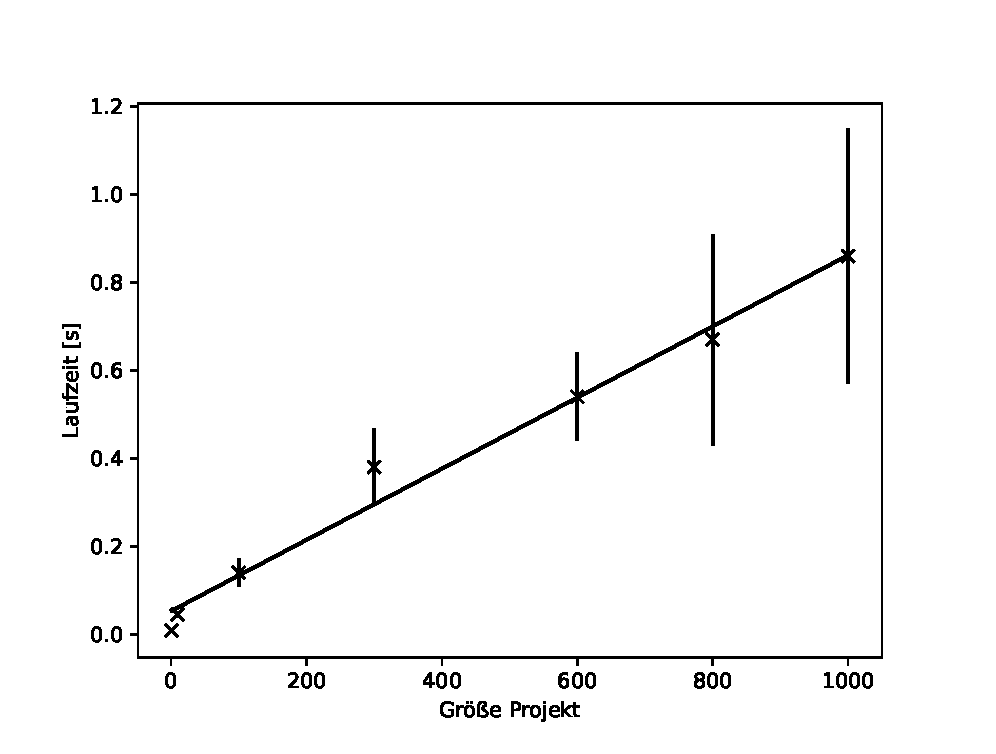
\includegraphics[width=\textwidth]{img/Runtime_Instrumenter.eps}
  \captionof{figure}{Laufzeit des Instrumenters}
  \label{Chap:Tracer-Sec:Laufzeit-Img:LaufzeitInstrumenter}
\end{minipage}
\hfill
\begin{minipage}{0.45\textwidth}
  \centering
  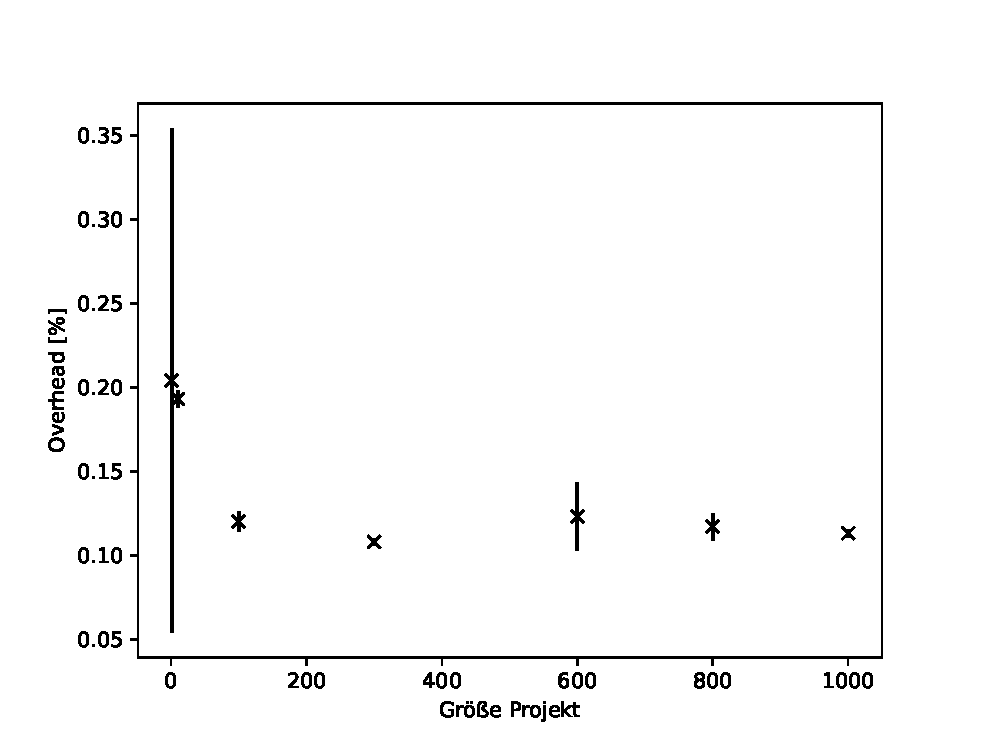
\includegraphics[width=\textwidth]{img/Runtime_Tracer.eps}
  \captionof{figure}{Prozentualer Overhead des Tracers ohne Analyse}
  \label{Chap:Trace-Sec:Laufzeit-Img:LaufzeitTracer}
\end{minipage}
Der abgebildete Graph zeigt die Laufzeit des Programms in $s$ abhängig von der 
Größe des Programms. Das Programm besteht dabei aus einem Testprogramm, welches 
alle möglichen Situationen mit Channels und Mutexen abbildet. Die Vergrößerung 
des Programmes wurde dadurch erreicht, dass die Datei mit dem Programmcode 
mehrfach in dem Projekt vorkam. Ein Projekt mit Größe $n$ besteht vor der 
Instrumentierung also 
aus $n$ Dateien, mit insgesamt $65n$ Zeilen von Code und $52n$ Ersetzungen
in dem AST. Die tatsächliche Laufzeit des Instrumenters auf einen 
Programm hängt schlussendlich natürlich von der tatsächlichen Größe des 
Projekt und der Verteilung der Mutex- und Channel-Operationen in dem Code ab.\\
\begin{table}[!h]
  \centering
  \begin{tabular}{|c|c|c|c|c|}
  \hline
  Projekt & LOC & Nr. Dateien & Nr. Ersetzungen & Zeit {[}s{]} \\ \hline
  ht-cat & $733$ & $7$ & $233$ & $0.013 \pm 0.006$ \\ \hline
  go-dsp & $2229$ & $18$ & $600$ & $0.029 \pm 0.009$ \\ \hline
  goker & $9783$ & $103$ & $4928$ & $0.09 \pm 0.03$ \\ \hline
  \end{tabular}
  \caption{Laufzeit des Instrumenters für ausgewählte Programme}
  \label{Chap:Tracer-Sec:Laufzeit-Tab:LaufzeitInstrumenter}
\end{table}
Zusätzlich wurde die Messung auch mit drei tatsächlichen Programmen 
durchgeführt. Die dort gemessenen Werte befinden sich in 
Tabelle~\ref{Chap:Tracer-Sec:Laufzeit-Tab:LaufzeitInstrumenter}. Gerade in 
Abhängigkeit von der Anzahl der Ersetzungen, stimmen die hier gemessenen Werte
mit denen in Abb.~\ref{Chap:Tracer-Sec:Laufzeit-Img:LaufzeitInstrumenter} gut 
überein, während es bei den anderen Parametern größere Abweichungen gibt.
Dies bestätigt dass der dominante Faktor für die Laufzeit des Programms 
die Anzahl der Ersetzungen in dem AST ist, und die Laufzeit linear von dieser 
abhängt.
\paragraph{Tracer} Folgend soll nun der Overhead des instrumentierten Codes 
im Vergleich zum originalen Code betrachtet werden.
Hierbei wird nur die Laufzeit eines Durchlaufs des eigentlichen Programs
(ohne Wiederholung aufgrund von Select), 
nicht aber der anschließenden 
Analyse betrachtet. Um den Overhead in Abhängigkeit von der Größe des Projektes messen 
zu können, wird das selbe Testprogramm betrachtet, welches bereits in der Messung 
für den Instrumenter verwendet wurde. Abb. \ref{Chap:Trace-Sec:Laufzeit-Img:LaufzeitTracer}
zeigt den gemessenen Overhead. Der durchschnittliche Overhead über alle gemessenen Werte 
liegt dabei bei $14 \pm 2\ \%$. Da der Overhead aber linear davon abhängt, 
wie groß der Anteil der Mutex- und Channel-Operationen im Verhältniss zu 
der Größe bzw. der Laufzeit des gesammten Programms ist, kann dieser Wert abhängig 
von dem tatsächlichen Programm start schwanken. Dies wird unteranderem klar, wenn man 
den Overhead für ht-cat ($9 \pm 3\ \%$) und go-dsp ($60\pm 18\ \%$) welche $51 \pm 21$ 
Prozentpunkte außeinander liegen. 
\extend{Laufzeit}

    
\chapter{Analyzer} \label{Chap:Implement}

Das folgende Kapitel soll sich nun mit der Implementierung der Analyze des in 
Kap.~\ref{Chap:Instrumenter-Sec:Trace} erstellten 
Trace befassen.

\section{Ablauf}
Um das Programm zu Analysieren wird der instrumentierte Code ausgeführt.
Besitzt es Select-Statements, dann wird es mehrfach durchgeführt, 
wobei jeweils eine andere, zufällige Ordnung für die Select-Cases 
betrachtet wird. Die betrachteten Ordnungen werden vor dem Durchlaufen 
der Programme erzeugt. Dabei kann vom Nutzer sowohl eine maximale 
Gesamtanzahl an Durchläufen angegeben werden. Zum anderen wird die 
Anzahl auch anhand der Dichte des Select-Cases beschränkt. Dazu wird 
eine neue, gültige Ordnung zufällig erzeugt und überprüft, ob diese 
Ordnung bereits zuvor erzeugt worden ist. Wenn sie neu ist, wird sie in 
die Liste der zu durchlaufenden Ordnungen eingefügt. Dabei wird gezählt,
wie oft eine Ordnung bereits zuvor erzeugt worden war. Auch für diesen 
Wert kann ein Maximalwert gesetzt werden.\\
Anschließend wird das Programm für jede der bestimmten Ordnungen analysiert.
Da das Programm gegebenenfalls mehrfach analysiert wird ist es wahrscheinlich, dass 
die selben Probleme mehrfach erkannt werden. Es ist daher nicht sinnvoll 
die Informationen direkt nach jedem Durchlauf auszugeben. Daher werden die 
Fehler gesammelt, und dabei jeweils gespeichert, bei welchen Durchlaufen die 
Fehler aufgetreten sind. Nach Abschluss aller Durchläufe werden die 
gesammelten Fehler vollständig ausgegeben.

\section{Aufzeichnung des Trace}
Der Trace wird wie in Kap.~\ref{Chap:Instrumenter-Sec:Trace}
beschriebenen erzeugt. Er wird dabei durch ein Slice von Slices 
gespeichert, wobei jeder Slice den Trace einer Routine 
speichert. Dazu wird für jedes Trace-Element ein Struct definiert, 
welches alle notwendigen Informationen speichert. Über ein Interface 
wird dafür gesorgt, dass diese Elemente alle in das Slice des Trace eingefügt
werden kann. Dabei wird über einen Mutex dafür gesorgt, dass nicht 
zwei Routinen gleichzeitig ein Element in den Trace einfügen können\\
Jeder Routine wird ein fortlaufender Wert eines atomaren Zählers zugeordnet. 
Um die interne Id einer Routine zu erhalten, und auf die dem Trace zugeordnete 
Id zuzuordnen wird eine externe Bibliothek GoId~\cite{goid} verwendet.\\
Auch die Ids für Channels und Mutexes werden durch laufende, atomare Zähler 
implementiert, welche in den Objekten für Channels und Mutexes gespeichert werden.

\section{Mutex} \label{Chap:Implement-Sec:Mutex}
Zuerst wird nach doppeltem Locking gesucht. Da ein doppeltes Locking immer 
zu einer blockade führt, kann es nur auftreten, wenn das letzte Element in 
dem Trace einer Routine eine Lock-Operation aber keine TryLock beschreibt. In diesem Fall wird 
der entsprechende Trace rückwerts durchlaufen, bis eine Operation auf dem 
selben Mutex gefunden wird. Handelt es sich dabei ebenfalls um eine 
Lock-Operation auf dem selben Mutex, bedeutet dies, dass ein Deadlock durch 
doppeltes Locking erkannt wurde. Dies ist allerdings nur der Fall, solange es 
sich nicht bei beiden Operationen um RLock-Operationen handelt. Wurde ein 
solcher Deadlock gefunden, wird eine eine entsprechende Nachricht zurückgegeben. 
Um potenzielle zyklische Deadlocks durch Mutexe erkennen zu können werden nun, wie in 
Kap.~\ref{Chap:Back-Sec:Prob-SubSec:Mutex} beschrieben, Lock-Bäume verwendet.
Diese werden basierend auf dem aufgezeichneten Trace aufgebaut. Dazu werden die Traces der 
einzelnen Routinen nacheinander durchlaufen. Für jede Routine wird eine Liste \texttt{currentLocks} aller 
Locks erzeugt, die momentan von der Routine gehalten werden. Die einzelnen Elemente des Trace einer 
Routine werden nun durchlaufen. Handelt es sich dabei um ein Lock Event eines Locks \texttt{x}, 
wird eine s.g. \texttt{Dependendency} erzeugt und gespeichert. Diese beinhaltet 
das Lock \texttt{x} sowie eine Liste aller von der Routine momentan gehaltenen 
Locks, dem s.g. \texttt{holdingSet hs}. Dieses entspricht gerade \texttt{currentLocks}. 
Diese \texttt{Dependendency} stellt also 
eine Menge von Kanten von in dem Lockgraphen der Routine da. 
Anschließend wird \texttt{x} in \texttt{currentLocks} eingefügt.
Ist das handelt es sich bei dem Element um ein unlock Event auf dem Lock \texttt{x}, dann wird das 
letzte Vorkommen von \texttt{x} auf \texttt{currentLocks} entfernt.\\
Nachdem der Trace einer Routine durchlaufen wurde, wird überprüft ob sich noch Elemente in 
\texttt{currentLocks} befinden. Ist dies der Fall, handelt es sich um Locks, welche zum Zeitpunkt der Terminierung 
des Programms noch nicht wieder freigegeben worden sind. Dies deutet darauf hin, dass die
entsprechende Routine nicht beendet wurde, z.B. weil das Programm bzw.\ die Main-Routine beendet wurden.
Dies kann einfach durch die entsprechende Logik des Programms zustande gekommen sein, es kann aber auch 
auf einen tatsächlich auftretenden Deadlock. In diesem Fall wird eine Warnung ausgegeben.\\
Ein potenzieller Deadlock gibt sich nun, wenn in diesem aus den Bäumen zusammengesetzten 
Graph ein Zyklus existiert.
Nicht alle Zyklen bilden dabei gültige Zyklen. Bum Beispiel muss darauf 
geachtet werden, dass nicht alle Kanten durch die selbe Routine erzeugt wurden, und dass in 
zwei, in dem Kreis hintereinander folgende Kanten der gemeinsame Knoten nicht beides mal durch eine 
R-Lock Operation durch Kanten verbunden wurde. Gültige Zyklen lassen sich durch 
dir folgenden Formeln charakterisieren.
\begin{align}
  &\forall\ i, j \in \{1,...,n\}\ \lnot (hs_i \cap hs_j = \emptyset) \rightarrow (i = j) 
  \tag{\ref{Chap:Implement-Sec:Mutex}.a}
  \label{Chap:Implement-Sec:Mutex.a}\\
  &\forall\ i \in \{1,...,n-1\}\ mu_i \in hs_{i+1} 
  \tag{\ref{Chap:Implement-Sec:Mutex}.b}
  \label{Chap:Implement-Sec:Mutex.b}\\
  &mu_n \in hs_{1} 
  \tag{\ref{Chap:Implement-Sec:Mutex}.c}
  \label{Chap:Implement-Sec:Mutex.c}\\
  &\forall i \in \{1,\ldots,n-1\}\ read(mu_i) \to (\forall mu\in hs_{i+1} (mu = mu_i) \to \lnot read(mu))
  \tag{\ref{Chap:Implement-Sec:Mutex}.d}
  \label{Chap:Implement-Sec:Mutex.d}\\
  &read(mu_n) \rightarrow 
  (\forall\ mu \in hs_{1}: (mu = mu_n) \to \lnot read(mu))
  \tag{\ref{Chap:Implement-Sec:Mutex}.e}
  \label{Chap:Implement-Sec:Mutex.e}\\
  &\makecell{\forall\ i, j \in \{1,...,n\}\ \lnot (i = j) \rightarrow 
  (\exists\ mu_1 \in hs_i\ \exists\ mu_2 \in hs_j ((mu_1 = mu_2) \rightarrow\\
  (read(mu_1) \land read(mu_2))))\phantom{123123123122131231231231223123}}
  \tag{\ref{Chap:Implement-Sec:Mutex}.f}
  \label{Chap:Implement-Sec:Mutex.f}
\end{align}
Dabei bezeichnet $mi_i$ den Mutex $hs_i$ das holdingSet der $i$-ten 
in dem Zyklus.\ (\ref{Chap:Implement-Sec:Mutex.a}) stellt sicher, dass das selbe 
Lock nicht in dem HoldingSet von zwei verschiedenen Routinen auftauchen kann.\
(\ref{Chap:Implement-Sec:Mutex.b}) und~(\ref{Chap:Implement-Sec:Mutex.c})
sorgen dafür, dass es sich bei der Kette tatsächlich um einen Zyklus handelt, 
dass also das Lock einer Dependency immer in dem HoldingSet
der nächsten Dependency enthalten ist und das Lock der letzten Routine 
wiederum im HoldingSet der ersten Routine liegt, um den Zyklus zu schließen.
(\ref{Chap:Implement-Sec:Mutex.d}) bis (\ref{Chap:Implement-Sec:Mutex.f})
beschäftigen sich mit dem Einfluss von RW-Locks auf die Gültigkeit von 
Zyklen. Auch wenn (\ref{Chap:Implement-Sec:Mutex.a}) bis~(\ref{Chap:Implement-Sec:Mutex.c})
erfüllt sind, ist dies dennoch keine gültige Kette, wenn sowohl
der Mutex $mu_i$ als auch der Mutex $mu$ in $hs_{i+1}$, 
für die $mu = mu_i$ gilt, beides Reader-Locks
sind, also Locks welche durch eine RLock-Operation erzeugt worden sind. 
Dass solche Pfade ausgeschlossen werden wird durch (\ref{Chap:Implement-Sec:Mutex.d})
und (\ref{Chap:Implement-Sec:Mutex.e}) sichergestellt.
(\ref{Chap:Implement-Sec:Mutex.f}) beschäftigt sich mit Gate-Locks. 
Dabei handelt es sich um Situationen, bei denen mehrere Teile des Programmcodes,
welche zu einem Deadlock führen könnten durch ein Lock umschlossen sind, 
in der Praxis also nicht gleichzeitig ausgeführt werden und somit einen Deadlock 
verhindern.
Die Regel besagt nun, dass wenn es einen Mutex gibt,
der in den HoldingSets zweier verschiedener Dependencies in dem Pfad vorkommt, so müssen
beide diese Mutexe Reader-Locks sein. Sind sie es nicht, handelt es sich um Gate-Locks, und
der entsprechende Pfad kann somit nicht zu einem Deadlock führen.

Für die Suche nach solchen Zyklen wird eine Depth-First-Search auf den gesammelten 
Dependencies ausgeführt. Dazu wird zuerst eine Dependency auf einen Stack gelegt. 
Der Stack entspricht immer dem momentan
betrachteten Pfad. Anschließend werden schrittweise weitere Dependencies auf den 
Stack gelegt, wobei darauf geachtet wird, dass aus jeder Routine immer nur maximal 
eine Dependency auf dem Stack liegt. Bevor eine Dependency zu dem Stack 
hinzugefügt wird, wird überprüft ob der durch den Stack betrachtete Pfad 
einen gültigen Pfad bilden würde, ob also (\ref{Chap:Implement-Sec:Mutex.a}), 
(\ref{Chap:Implement-Sec:Mutex.b}), (\ref{Chap:Implement-Sec:Mutex.d}) und 
(\ref{Chap:Implement-Sec:Mutex.f}) immer noch gelten würden. Ist dies nicht
der Fall, so wird die Dependency nicht auf den Stack gelegt. Werden die 
Regeln hingegen erfüllt, dann wird überprüft, um der Stack nun einen gültigen
Zyklus enthält, also auch (\ref{Chap:Implement-Sec:Mutex.c}) und (\ref{Chap:Implement-Sec:Mutex.e})
gültig sind. In diesem Fall wurde ein potenzielles Deadlock gefunden, und dies 
ausgegeben. Andernfalls werden weiter Dependency auf dem Stack hinzugefügt. 
Dies wird wiederholt, bis es keine Dependency mehr gibt, die auf den Stack VaT
gelegt werden könnte. In diesem Fall werden per Backtracking Dependencies 
von dem Stack entfernt, so dass andere Pfade ausprobiert werden können.
Dies wird so lange durchgeführt. Bis alle gültigen Kombinationen durchprobiert 
worden sind.

\section{Channels}\label{Chap:Analyse-Sec:Channel}
Die Analyse des Programs zur Erkennung und Beschreibung von durch Channels ausgelösten 
Problemen läuft in mehreren Schritten ab. Zuerst werden die Vectorclock-Informationen 
der einzelnen Operationen bestimmt und mit diesen ein vectorclock-annotated Trace 
(VaT) erzeugt. Basierend auf diesen sucht der Analyzer nach potenziellen 
Situationen, welche zu blockenden Message-Bugs oder nicht gelesene
Nachrichten auf gebufferten Channels führen können. Zum Schluss 
wird nach Situationen gesucht, bei denen es zu einem Send auf einen 
geschlossenen Channel kommen kann, da solche Situationen zu Laufzeitfehlern 
führen, welche den Abbruch eines Programms zur Folge haben.
Receives auf geschlossenen Channels werden nicht betrachtet, da diese 
lediglich einen Null-Wert zurückgeben und nicht blocken, somit also nicht 
zu Laufzeitfehlern führen. 

\paragraph{Bestimmung des vectorclock-annotierten Trace VAT}
Basierend auf dem aufgezeichneten Trace soll nun ein vectorclock-annotierter Trace 
(VAT) erzeugt werden. Dieser besteht aus einer Reihe von \texttt{vcn}'s, 
welche jeweils eine Send-, Receive- oder Close-Operation repräsentieren.
Andere Operation, wie z.B. signal-wait werden zwar bei der Berechnung der Vectorclocks 
beachtet, allerdings nicht in den VAT aufgenommen, da sie für die weitere 
Analyse nicht benötigt werden. Ein \texttt{vcn} beinhaltet dabei die Channel-Id,
die Routine, ob es sich um Send- oder Receive handelt (bei Close beliebig gesetzt),
ein Counter für die Anzahl der bereits erfolgreich abgeschlossenen Send- bzw.
Receive-Operationen bei der Ausführung des Send- oder Receive (bei Close -1), 
die Position der Operation im Programmcode
sowie die Pre- und Post-Vectorclocks der Operation. Eine Close Operation 
wird dabei dadurch erkannt, dass die Pre- und Post-Vectorclocks übereinstimmen.

Bevor der eigentliche VAT erzeugt wird werden erst die Vectorclocks zu allen
Zeitpunkten bestimmt. Dazu wird für jede Routine eine Vectorclock initialisiert. 
Anschließend werden die Elemente in der Reihenfolge durchlaufen, in der sie 
in den Trace eingefügt wurden, also aufsteigend sortiert nach dem Timestamp 
der Trace-Elemente. Für jeden Zeitpunkt wird nun eine Vectorclock berechnet,
wobei für jeden Timestamp immer diejenige Vectorclock gespeichert wird, die 
der Vectorclock entspricht, auf welcher die entsprechende Operation ausgeführt wurde.
Für die Berechnung der Vectorclocks werden signal-wait Paare wie das Senden 
einer Nachricht von signal nach wait betrachtet.\\
Für send (post) und Signal bzw. Receive (post) und Wait werden nun die Vectorclocks 
aktualisiert.
Für Send und Signal wird lediglich der eigene Timestamp in der eigenen 
Vectorclock um eins erhöht. Für die Aktualisierung bei einem Receive oder Wait 
wird die Vectorclock zur Zeit von Send oder Signal benötigt. Da diese in jedem 
Fall vor dem Receive oder Wait erzeugt worden sind, wurden sie bereits berechnet.
Da für die Receive-Elemente in dem Trace die Zeitstempel der Send-Operationen 
gespeichert sind, ist eine eindeutige Zuordnung der Send- und Receive-Statements 
möglich. Für die Signal- und Wait-Elemente ist jeweils die Id der neu erzeugten 
Routine gespeichert. Es ist also auch hier eine eindeutige Zuordnung möglich. 
Die Vectorclock der Send- bzw. Signal-Operation kann also immer eindeutig bestimmt 
werden und die Vectorclock somit wie in Kap.~\ref{Chap:Analyze-Sec:Channel-SubSec:Dangling}
beschrieben aktualisiert werden.\\
Für alle anderen Element, also alle Pre-Elemente, Close-Operationen und Mutex-Operationen 
werden die Vectorclocks lediglich kopiert.

Nach der Berechnung der Vectorclocks kann nun der VAT bestimmt werden. 
Dazu wird nun der Trace für die einzelnen Routinen durchlaufen. Bei jedem 
Pre- und PreSelect-Element wird eine \texttt{vcn} erzeugt. Dazu wird der restliche Trace 
der selben Routine durchlaufen um das zugehörige Post-Element zu finden. 
Wird diese gefunden wird 
das \texttt{vcn} erzeugt, wobei die Pre- und Post-Vectorclock über den 
Zeitstempel der Pre- und Post-Elemente aus der Liste der Vectorclocks 
übernommen wird.
Wird kein Post-Element gefunden, handelt es sich also um ein hängendes Event, 
wird die Pre-Vectorclock auf die Vectorclock des Pre-Events und alle Elemente 
der Post-Vectorclock auf \texttt{maxInt}, als den maximal möglichen Wert 
gesetzt. In diesem Fall wird der entsprechende Channel außerdem in die Liste der
hängenden Channels aufgenommen. 
\\
Für Close-Elemente gibt es nur ein Element in dem Trace. Aus diesem Grund 
besitzt das Element nur eine Vectorclock. Pre- und Post-Vectorclock werden 
dabei auf die gleiche Vectorclock gesetzt.

\paragraph{Erkennung pottenzieller Communication-Bugs}
Basierend auf dem VAT können nun tatsächlich aufgetretene oder potenzielle 
Communication-Bugs erkannt werden. Dabei wird nach Channel-Operationen 
gesucht, welche bei bestimmten Abläufen keine gültigen Kommunikationspartner
besitzen. Dies führt zu einem blocken Bug, durch das warten auf 
Sends oder Receives oder das Senden von Nachrichten auf gebufferten 
Channels, ohne das die Nachricht jemals ausgelesen wird.\\  
Zuerst werden basierend auf dem VAT alle potenziellen Kommunikationspartner 
für Send-Receive Paare bestimmt.
Zur Suche nach alternativen Kommunikationspartner von ungebufferten Channels
werden alle Kombinationen
von zwei Elementen in dem VAT betrachtet. Dabei werden all diejenigen 
Elemente verglichen, bei welchen beide Operationen auf dem selben Channel 
ausgeführt werden und eines der 
Elemente ein Send- und das andere eine Receive-Operation ist. Zwei Operationen
werden als potenzielle Kommunikationspartner angesehen, wenn die Pre- oder
Vectorclocks der beiden 
Operationen unvergleichbar sind.\\
Für den gebufferten Channel müssen Send- und Receive nicht 
gleichzeitig ausgeführt werden. Aus diesem Grund müssen die Vectorclocks 
nicht unvergleichbar sein. Um mögliche Kommunikationspartner zu erkennen 
werden daher 
die in Abschnitt~\ref{Chap:Theo-Sec:Analyze-SubSec:Channel} beschriebenen 
Werten für jedes Element in dem VAT ermittelt. Dazu werden alle Send- mit allen 
Send- und alle Receive- mit allen Receive-Operationen verglichen 
und dabei überprüft, ob die Pre- und Post-Vectorclocks eine Happens-Before 
Relation bilden, bzw. ob sie unvergleichbar und damit nebenläufig sind. 
Für jede Operation wird dabei gezählt, mit wie vielen anderen Operationen 
dies der Fall ist.
Für die Bestimmung der potenziellen Kommunikationspartner wird nun 
für jedes Paar von Send-Receive-Operationen auf dem selben Channel 
überprüft, 
ob die Formeln~(\eqref{Form:1}) und~(\eqref{Form:2}) 
erfüllt. In diesem Fall wird angenommen, dass die beiden Operationen
miteinander Kommunizieren können.\\
Basierend auf diesen möglichen Kommunikationspartnern werden nun alle möglichen
Kommunikationsabläufe betrachtet. Für die Betrachtung aller Abläufe 
wird Backtracking verwendet. Zuerst wird schrittweise rekursiv für jede Send-Operation 
in dem Trace eine potenzielle Receive-Operation als Kommunikationspartner 
in einen partiellen Kommunikationsablauf eingefügt, sofern die 
Receive-Operation einen gültigen Kommunikationspartner bildet. Ein Receive 
ist ein potenzieller Kommunikationspartner, wenn eine Kommunikation 
basierend auf dem VAT möglich ist, die Receive-Operation noch von keiner 
anderen Send-Operation als Partner verwendet wird. Besitzt ein solcher Pfad 
einen Kommunikationspartner für jedes Send-Statement in dem Trace, bedeutet dies, 
dass der entsprechende Ablauf nicht zu einem Bug führen kann. Ist es hingegen 
nicht möglich einem Send ein gültiges Receive zuzuordnen, dann führt der 
entsprechende Ablauf zu einem potenziellen Bug. Bevor dieser zurückgegeben 
werden kann muss erst noch überprüft werden, ob es sich um eine 
gültige Ausführungsordnung handelt, wie in Abschnitt~\ref{Chap:Theo-Sec:Analyze-SubSec:Channel} 
beschrieben. Ist diese der Fall, wird eine entsprechende Nachricht ausgegeben, 
welche die Operation, welche zu dem Bug führt, sowie den partiellen
Ausführungspfad, bei welchem der Bug auftreten kann, enthält.\\In beiden 
Fällen, in denen das Hinzufügen weiterer Send-Operationen nicht mehr möglich ist 
wird nun Backtracking verwendet, um die weiteren Ausführungspfade zu betrachten.
Da die Reihenfolge, mit welcher die Send-Statements in den partiellen 
Ausführungspfad eingefügt werden werden, insbesondere welche Operation als erstes 
betrachtet wird, Auswirkung auf die Detektion von Problemen haben kann, 
wird das ganze für jede zyklische Permutation der Send-Operationen wiederholt. \\
Das Ganze wird anschließenden ein zweites Mal ausgeführt, wobei die Rollen 
von Send und Receive hierbei vertauscht sind. Es wird also für jedes Receive 
eine Send-Operation gesucht. 

\paragraph{Erkennung von potenziellem Senden auf geschlossenem Channel}
Für die Suche nach Situationen, die dazu führen können, dass auf einem 
geschlossenen Channel gesendet wird, werden die Vectorclock aller in dem 
Trace vorhandenen Close-Operationen mit den Vectorclocks aller Send-Operationen
auf dem selben Channel verglichen. Ist mindestens eine der beiden Vectorclocks 
unvergleichbar, dann nimmt das Programm an, das eine Send-Operation auf 
einen geschlossenen Channel möglich ist, und gibt eine entsprechende 
Warnung zurück. Es kommt auch zu einem Send auf einem geschlossenen Channel, 
wenn die Vectorclock der Close-Operation streng vor den Vectorclocks 
der Send-Operation sind. In diesem Fall kommt es aber in jedem Fall zu einem 
Send auf einen geschlossenen Channel und damit zu einem Laufzeitfehler, 
welcher durch den Detektor aufgefangen und erkannt wird.


\section{Beispiel}
In Anhang~\ref{Appendix-2} findet sich ein Beispielprogramm sowie die erhalten Ausgabe. 
    \chapter{Auswertung}\label{Chap:Eval}
Im Folgenden soll betrachtet werden, wie gut der beschriebene Detektor 
in der Lage ist, Situationen wie in Abschnitt~\ref{chap:background-sec:Prob}
beschrieben zu erkennen. Dabei werden sowohl künstlich konstruierte 
Situationen, als auch tatsächliche Programme betrachtet. Für die Betrachtung 
tatsächlicher Programme werden Programme aus Goker~\cite{gobench}
verwendet. Dieses besitzt eine Sammlung von Programmteilen mit 
Concurrency-Bugs aus 9 
großen open-source Anwendungen wie z.B. Kubernetes und Moby. 
Beschreibungen der Probleme, sowie die Ergebnisse des Detektors befinden in 
Anhang~\ref{Appendix-1}.

\section{Standardprogramme}
Für die Analyse wurden insgesammt 35 Standartprobleme betrachtet. 
Dabei wurde überprüft, ob der Detektor in der Lage ist, das in dem 
Programm erhaltene Problem richtig zu erkennen, bzw.~zu erkennen wenn 
die vorliegende Situation nicht zu einem Problem führen kann. Eine 
tabellarische Beschreibung der betrachteten Situationen, sowie der Ergebnisse 
des Detektors ist in Tab.~\ref{App-Stand} in Anhang~\ref{Appendix-1} aufgeführt.\\\\
Von den 43 Programmen konnten 39 korrekt kategorisiert werden. Dabei 
bestehen 18 Probleme aus Problemen mit Mutexen,
18 aus Problemen mit Channel und 7 mit einem 
Mix aus Mutexen und Channel. Abbildungen~\ref{Chap:Eval-Sec:Stand-Fig:Total}
bis~\ref{Chap:Eval-Sec:Stand-Fig:Mix} geben an, welcher Anteil der 
Betrachteten Standartprobleme korrekt erkannt wurde.\\\\
Für Programme, bei denen der Fehler auf die Verwendung von Mutexen 
basiert, konnten 17 der 18 Probleme richtig kategorisiert werden. 
Dies entspricht ca. $94.4\%$.\\
Bei den Programmen, bei welchen es durch Channel zu Problemen kommen kann, 
konnten ebenfalls 17 der 18 Programme.\\
Bei Programmen, welche sowohl Mutexe als auch Channels verwenden liegt 
die Erfolgsquote mit 5 aus 7 ($71.4\%$) am niedrigstem. Da der Detektor 
zwei verschiedene Methoden verwendet, um Probleme mit Mutexen und Probleme 
mit Channels zu erkenne, aber keine direkte Methode für die Erkennung
von Problemen besitzt, welche durch eine Kombination der beiden entstehen, 
werden solche Situationen nicht direkt erkannt. Sie werden nur dann erkannt, 
wenn sie dazu führt, dass einer der beiden Mechanismen sie erkennen 
kann. Es ist daher nicht verwunderlich, dass hierbei eine höhere Fehlerquote 
betrachtet werden kann, als wenn man die beiden Situationen einzeln
betrachtet.\\
Insgesamt hat der Detektor für die betrachteten Programme eine 
Trefferwahrscheinlichkeit von $90.7\%$. \\
Es sei noch dazu gesagt, dass die betrachteten Programme immer so implementiert 
worden sind, dass die entsprechenden Situationen auch in dem Durchlauf 
auftreten. Es ist allerdings auch möglich, dass Situationen bei den Durchläufen 
nicht durchlaufen werden, z.B. wenn sie sich ein einem Konditionellen 
Block (If) befinden, bei welchem die Bedingung während keinem der Durchläufe 
wahr wird. Da die entsprechenden Operationen somit nicht aufgezeichnet 
werden können, ist es demnach logischerweise auch nicht möglich, dass der 
Detektor die entsprechenden Situationen erkennt.




\begin{minipage}{0.45\textwidth}
  \centering  
  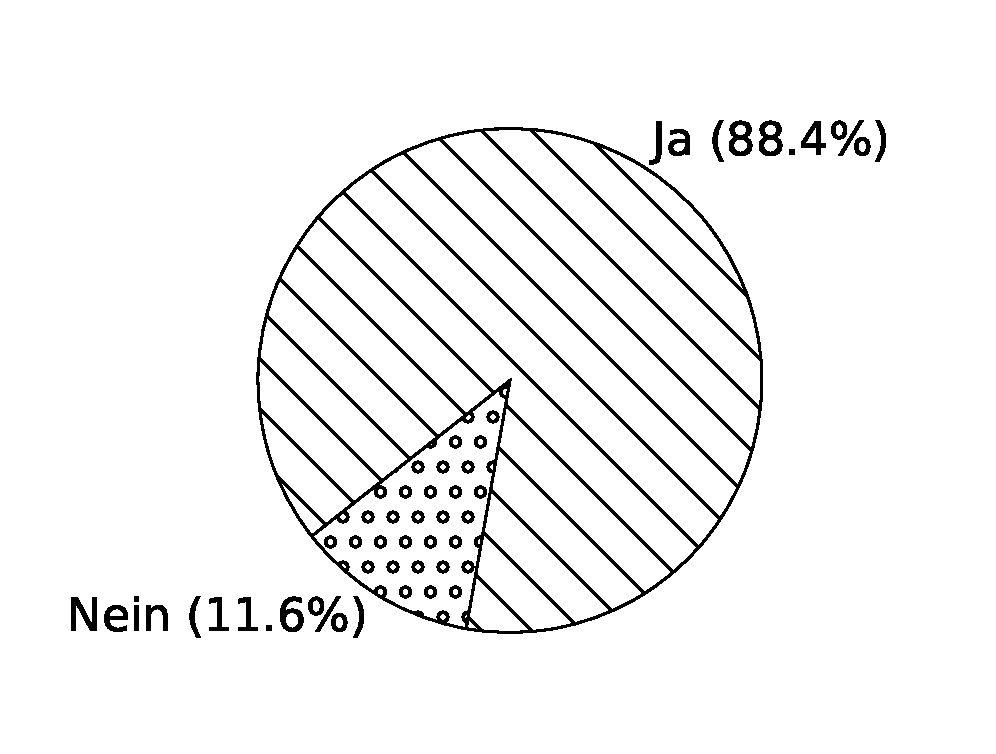
\includegraphics[width=0.8\textwidth]{img/pi_standard_total.eps}
  \captionof{figure}{Verteilung der Ergebnisse für Standardprogramme}
  \label{Chap:Eval-Sec:Stand-Fig:Total}
\end{minipage}
\hfill
\begin{minipage}{0.45\textwidth}
  \centering
  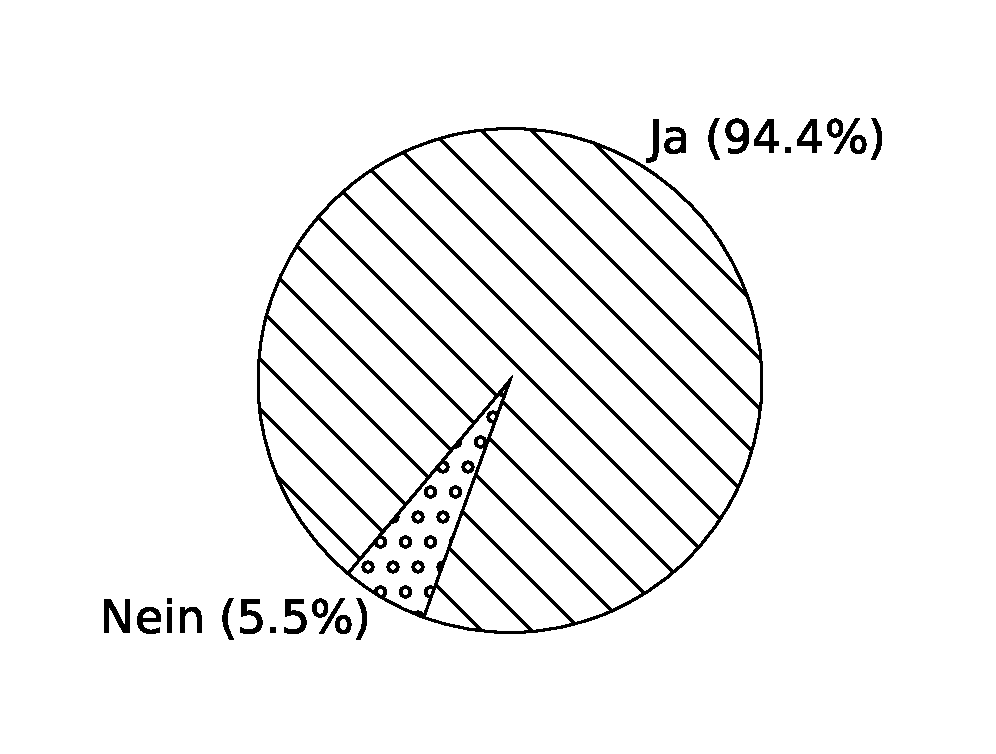
\includegraphics[width=0.8\textwidth]{img/pi_standard_mutex.eps}
  \captionof{figure}{Verteilung der Ergebnisse für Standardprogramme mit Mutexen}
  \label{Chap:Eval-Sec:Stand-Fig:Mutex}
\end{minipage}
\begin{minipage}{0.45\textwidth}
  \centering  
  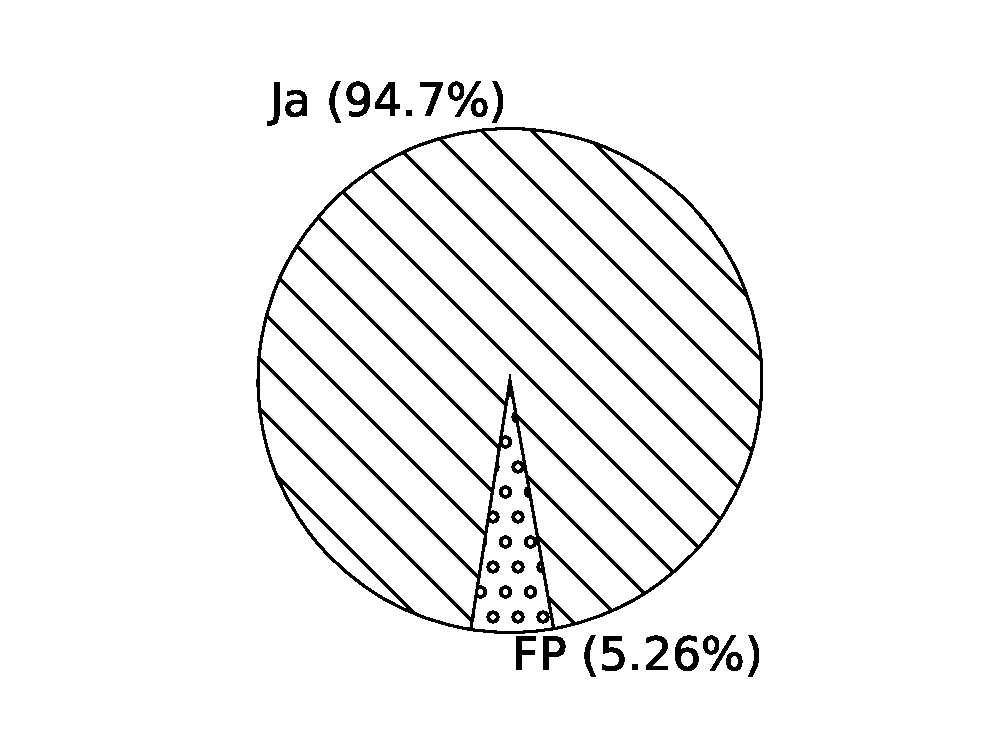
\includegraphics[width=0.8\textwidth]{img/pi_standard_channel.eps}
  \captionof{figure}{Verteilung der Ergebnisse für Standardprogramme mit Channel}
  \label{Chap:Eval-Sec:Stand-Fig:Channel}
\end{minipage}
\hfill
\begin{minipage}{0.45\textwidth}
  \centering
  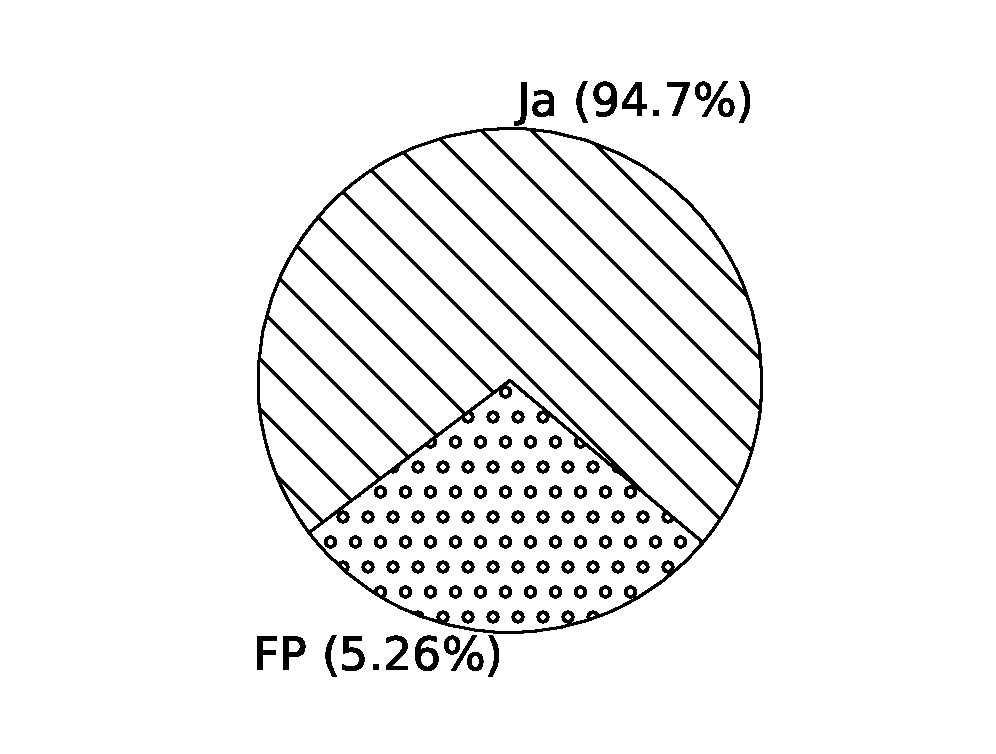
\includegraphics[width=0.8\textwidth]{img/pi_standard_mix.eps}
  \captionof{figure}{Verteilung der Ergebnisse für Standardprogramme mit Mutexen und Channel}
  \label{Chap:Eval-Sec:Stand-Fig:Mix}
\end{minipage}

\section{GoKer}
Für die Analyse wurden insgesamt 34 Programme betrachtet. Die betrachteten 
Programme und deren Ergebnisse befinden sich in Tab.~\ref{App-Goker} 
in Anhang~\ref{Appendix-1}. Von den Programmen betrafen 15 die 
Verwendung von Resource wie Mutexen (14 korrekt erkannt), 11 die 
Verwendung von Kommunikationen (10 korrekt erkannt) und 8 eine Kombination aus Mutexen und 
Channel (7 korrekt erkannt).
Die Erfolgsraten des Detektors für die Programme aus GoKer 
(Abb.~\ref{Chap:Eval-Sec:Goker-Fig:Total} bis~\ref{Chap:Eval-Sec:Goker-Fig:Mix})
stimmen dabei in etwa mit denen der Standardprogramme überein.
Für die Analyse wurden dabei nur solche Programme ausgewählt,
welche basieren auf ihrer Beschreibung für den Detektor theoretisch erkennbare 
Situation enthielt. Situationen, welche sich auf andere Concurrency-Bugs,
z.B. Race-Conditions bezogen wurden nicht betrachtet. 
Die Betrachtung der Programme aus Goker hat einen Nachteil der hier 
verwendeten Methode, bzw. der Implementierung deutlich gemacht.
Der Instrumenter ist nur in der Lage den vorliegenden Code zu instrumentieren. 
Es kann aber vorkommen, dass in einem Programm externe Funktionen 
verwendet werden, welche Mutexe oder Channel als Parameter oder 
Rückgabewerte besitzen. Da bei der Instrumentierung Mutexe und Channel 
durch eingens implementierte Objekte ersetzt werden, externe Funktionen 
aber nicht entsprechend Instrumentiert werden können kommt es 
hierbei zu Compiler-Fehlern. Die entsprechenden Programme sind daher nicht 
Lauffähig und können somit auch nicht analysiert werden. Programme aus GoKer, 
bei denen dies der Fall war wurden für die Analyse nicht betrachtet. 

\begin{minipage}{0.45\textwidth}
  \centering  
  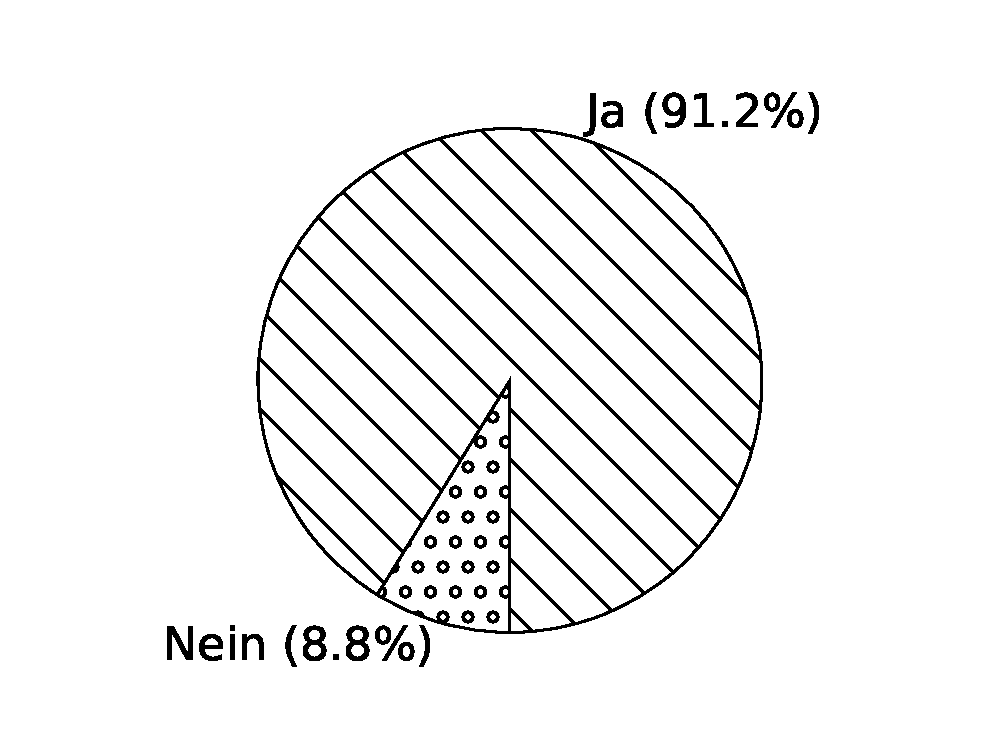
\includegraphics[width=0.8\textwidth]{img/pi_goker_total.eps}
  \captionof{figure}{Verteilung der Ergebnisse für Programme aus GoKer}
  \label{Chap:Eval-Sec:Goker-Fig:Total}
\end{minipage}
\hfill
\begin{minipage}{0.45\textwidth}
  \centering
  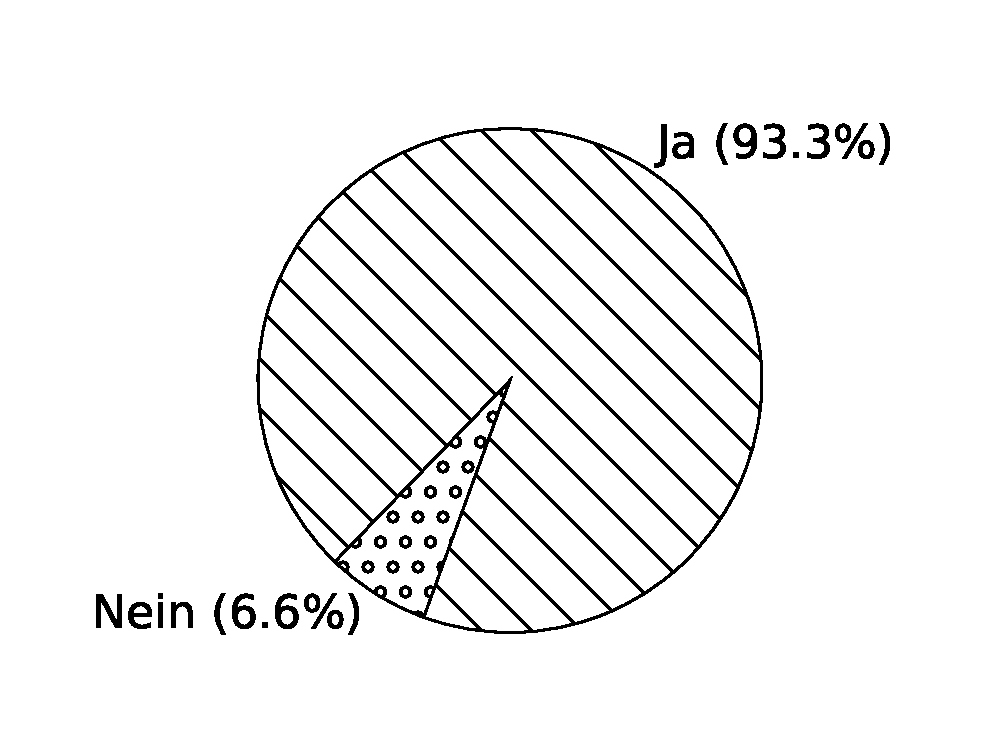
\includegraphics[width=0.8\textwidth]{img/pi_goker_mutex.eps}
  \captionof{figure}{Verteilung der Ergebnisse für Programme aus GoKer mit Mutexen}
  \label{Chap:Eval-Sec:Goker-Fig:Mutex}
\end{minipage}
\begin{minipage}{0.45\textwidth}
  \centering  
  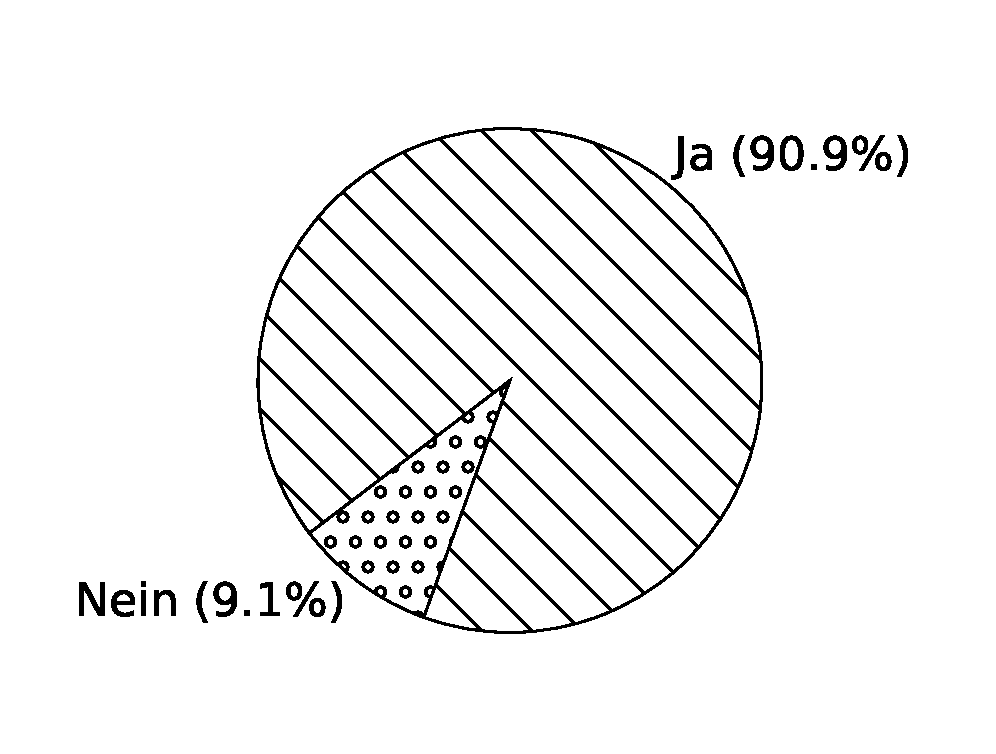
\includegraphics[width=0.8\textwidth]{img/pi_goker_channel.eps}
  \captionof{figure}{Verteilung der Ergebnisse für Programme aus GoKer mit Channel}
  \label{Chap:Eval-Sec:Goker-Fig:Channel}
\end{minipage}
\hfill
\begin{minipage}{0.45\textwidth}
  \centering
  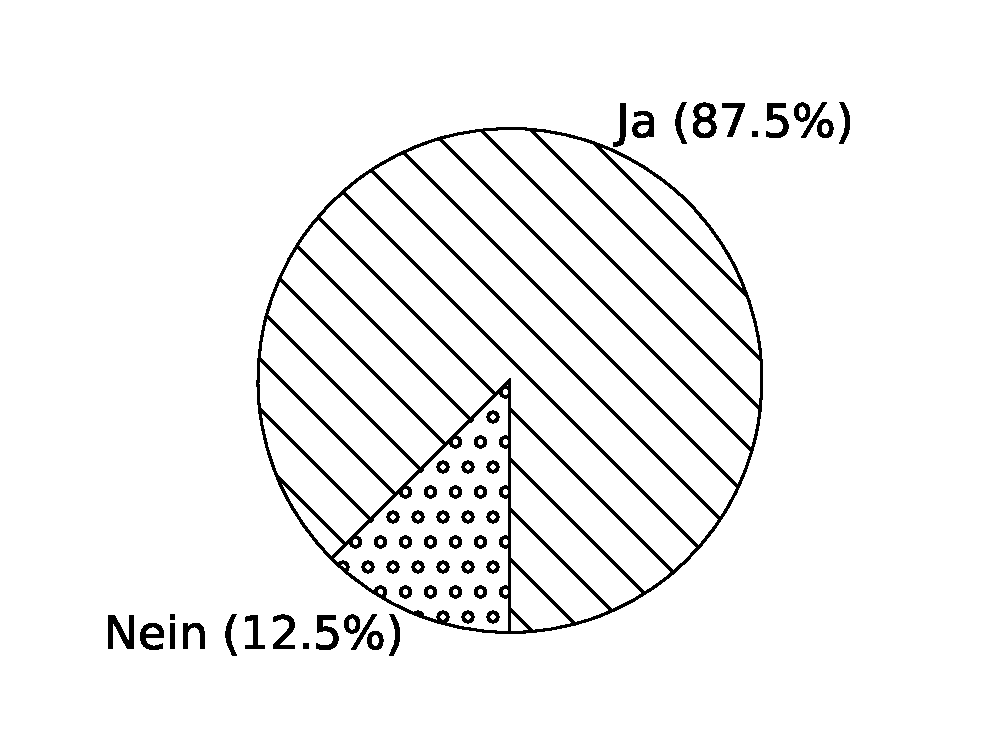
\includegraphics[width=0.8\textwidth]{img/pi_goker_mix.eps}
  \captionof{figure}{Verteilung der Ergebnisse für Programme aus GoKer mit Mutexen und Channel}
  \label{Chap:Eval-Sec:Goker-Fig:Mix}
\end{minipage}

\section{Probleme} \todo{Anderer Name}
\todo{Situationen, welche nicht betrachtet werden (z.B. in If, nach blockierender situation)}
\todo{Kommunikationene, welche in anderem Ablauf nicht möglich sind?}

Aufgrund der Funktionsweise des Implementers und der Analyse kann der Detektor 
momentan nur auf Probleme angewendet werden, welche durch 
\texttt{go build} kompiliert und anschließend direkt ausgeführt werden können.
Aus diesem Grund ist die direkte Anwendung des Detektors auf viele größere Programm 
in seinem momentanen Stand nicht möglich. 
    \chapter{Zusammenfassung}\label{chap:conclusion}
Ziel dieser Arbeit war es einen Detektor für von Mutexen 
und Channels erzeugte Concurrency-Bugs zu entwickeln und zu implementieren.\\
Der implementierte Detektor vereinigt und erweitert dabei verschiedene Methoden 
zur Erkennung solcher Probleme. Der Detektor erzeugt dynamisch einen Trace 
eines vorliegenden Programms, welcher im Anschluss analysiert werden kann.
Für Deadlocks durch Mutexe werden dabei unter anderem Lock-Bäume verwendet. 
Für Channel-Operationen wird der Trace mit Vector-Clocks erweitert, 
durch welche Schlussfolgerungen auf mögliche Kommunikationspartner oder 
das potenzielle Senden auf geschlossene Channels erkannt werden. 
Bei der Anwendung auf konstruierte Probleme und tatsächliche Programme 
ist der so entwickelte Detektor in der Lage knapp $91\%$ aller betrachteten 
Situationen richtig zu kategorisieren. 
\todo{Bisschem mehr}
    \chapter{Acknowledgments}
\todo{Acknowledgments schreiben}
    \listoffigures
    \listoftables
    % \listofalgorithms
    % \lstlistoflistings
    
    % If you want a list of your ToDos at the end of the document
    % don't forget to remove before submission!
    % place it somewhere in the document
\chapter*{ToDo Counters}
\todo{Remove ToDo Counter List}\\
\newcounter{ct}%
To Dos: \arabic{todos}; \hspace{1em}%
\setcounter{ct}{0}%
\whiledo{\value{ct} < \value{todos}}%
{%
	\stepcounter {ct}%
    \ref{todo \thect}%
	\ifnum\value{ct} = \value{todos}{}\else{, }\fi
}

Parts to extend: \arabic{extends}; \hspace{1em}%
\setcounter{ct}{0}%
\whiledo {\value{ct} < \value{extends}}%
{%
	\stepcounter {ct}%
	\ref{extend \thect}%
	\ifnum\value{ct} = \value{extends}{}\else{, }\fi
}

Draft parts: \arabic{drafts}; \hspace{1em}%
\setcounter{ct}{0}%
\whiledo {\value{ct} < \value{drafts}}%
{%
	\stepcounter {ct}%
	\ref{draft \thect}%
	\ifnum\value{ct} = \value{drafts}{}\else{, }\fi
}
 

    \bibliographystyle{ieeetr}
    \bibliography{bib/references,bib/sources}
    % bibliography is not in the table of contents per default, add it manually
    % enable the \renewcommand for german header
    \renewcommand{\bibname}{Literaturverzeichnis}
    \addcontentsline{toc}{chapter}{Literaturverzeichnis}
    \newpage
    \thispagestyle{empty}
    \mbox{}
  
\end{document}
